\chapter{Coffee Time Analysis}
\label{ch:analysis}
In this chapter, the specification of the implemented application is outlined. The analysis of similar applications was made to obtain ideas.  After analysis, the low fidelity prototype was created to outline the first vision of the final application. Next, the high-fidelity prototype, along with Nielsen's heuristics analysis and user testing, were made. At the end of the chapter, considered tools and services which are used to implement the application are briefly described. 
% ----- % ----- % ----- % ----- % ----- % ----- % ----- % ----- % ----- % ----- % ----- % ----- % ----- % ----- %
\section{Considered Application}
Coffee Time is an application focused on searching nearby cafes. Users should be able to search and find nearby cafes around them and decide which establishment to visit. Each cafe is displayed with information such as distance, user's reviews, photos, opening hours and more. 

Added value to this standard information is a feature so-called ``the tags''. These tags are user-added additional info which describes more precisely what given cafe offer or for instance if that cafe allows pets inside. 

The set of tags is defined, and users can add these tags to the~cafe.  Each tag can be reviewed by other users. These reviews are done through ``like'' and ``dislike'' functionality. The~purpose of tag's reviews is to prevent outdated from information or misleading information.  

The example of such review can be ``User visited cafe which has tag 'dog friendly', but unfortunately this information was incorrect. Consequently, the~user decided to open the~application and review the~cafe's tag 'dog friendly' with dislike.''

Together with likes and dislikes, each tag has a computed score.  Each like gives to score plus one and as an opposite, dislike minus one. 
If any tags reach the score to~-4, the~tag is removed from the cafe, more precisely is not shown anymore to users. 
If such removed tag is proposed by any user again, it obtains "like" review. Thus score is incremented to -3 and is shown again. 

The application is location-based and offers a map view to support the~convenience user experience. Any cafe can be marked as user's favourite to~give a faster way to find cafe whenever the user wants. 

In conclusion, Coffee Time is application focused on one domain -- searching nearby cafes in order to know where to~go to~study, talk with friends or~for example have a great coffee. The application should be simple to use with a clean user interface. 
% ----- % ----- % ----- % ----- % ----- % ----- % ----- % ----- % ----- % ----- % ----- % ----- % ----- % ----- %
\section{Use Cases}
From the specification above, the use cases and use case scenarios were formed. The~use cases diagram is listed in \cref{fig:use_case} and shows every use cases from the~user perspective. Technically there is the role of application administrator who can check control back-end or available application's tags, but it is skipped due to the lack of importance from application perspective. 

\begin{figure}[htp]
    \centering
    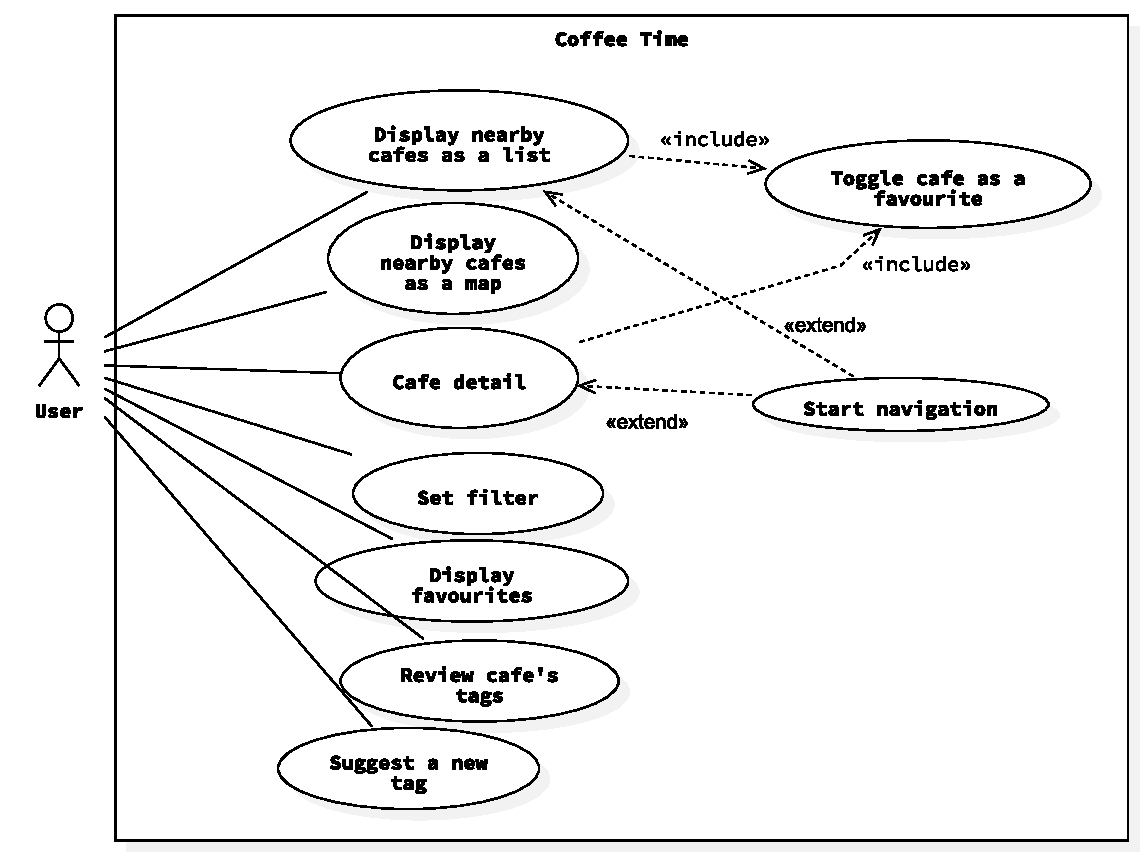
\includegraphics[width=\linewidth]{img/analysis/use_case.pdf}
    \caption{Application's use case diagram}
    \label{fig:use_case}
\end{figure}

As shown on diagram, the application has several use cases

\begin{itemize}
    \item UC1: Display nearby cafes as a list.
    \item UC2: Display nearby cafes as a map.
    \item UC3: Start navigation.
    \item UC4: Toggle cafe as a favourite.
    \item UC5: Setting the filter.
    \item UC6: Display favourite cafes.
    \item UC7: Review the cafe's tags.
    \item UC8: Suggest a new tag.
\end{itemize}

\subsection{UC1: Display Nearby Cafes As a List}
User can display nearby cafes in the form of the list view. The result is filtered by setting a filter, which can be altered by \textit{UC5}.

\textbf{Pre-Conditions} The user must be on the cafe list screen.

\newpara
\textbf{Basic Flow}

\begin{enumerate}
    \item User launch Coffee Time and lands on cafe list.
    \item Cafe list shows nearby cafes around him. Each cafe is displayed in the form of a card.
    \item User can pull the list down to refresh results. 
    \item User taps on cafe's card and is redirected to the detail view.
\end{enumerate}

\textbf{Alternative flow 1} The user launch navigation to the selected cafe.

% -------------

\subsection{UC2: Display Nearby Cafes as Map}
User can display nearby cafes in the form of the map view. Each cafe is shown as a map marker.

\textbf{Pre-Conditions} The user must be on the map screen.

\newpara
\textbf{Basic Flow}

\begin{enumerate}
    \item User launch application and change screen to map view. 
    \item Nearby cafes are shown as markers.
    \item The user taps on the marker and is redirected to the detail screen.
\end{enumerate}

\textbf{Alternative flow 1} The user taps anywhere on the map to display nearby cafes on the selected location.

% -------------

\subsection{UC3: Start navigation}
Use case allows starting navigation to selected cafe through native navigation applications.

\textbf{Pre-Conditions} The navigation services must be enabled.

\newpara
\textbf{Basic Flow}

\begin{enumerate}
    \item The user selects the cafe.
    \item The user selects navigate action. 
    \item The system request to open navigation application is opened. 
    \item User enables navigation and is redirected to navigation application. 
\end{enumerate}

\textbf{Alternative flow 1} The user dismisses navigation request and cancels navigation.

% -------------
\subsection{UC4: Toggle cafe as a favourite}
Each cafe can be marked as a favourite to faster future access. 

\textbf{Pre-Conditions} The cafe must be loaded, so that it is visible to the~user. The~user must be either on the~cafe list screen, detail screen or favourite screen. 

\newpara
\textbf{Basic Flow}

\begin{enumerate}
    \item User has a cafe which wants to toggle as a favourite.
    \item User toggles cafe as a favourite.
\end{enumerate}

% -------------

\subsection{UC5: Setting the filter}
User changes the filter settings to filter out the cafe results.

\textbf{Pre-Conditions} There are results to filter.

\newpara
\textbf{Basic Flow}

\begin{enumerate}
    \item User opens filter settings screen.
    \item If it is suitable user changes results ordering from ``by distance'' (default) to ``by popularity''.
    \item If it is suitable user changes opening hours filter.
    \item Add tags to filter by, if any.  
    \item Returns back to the previous screen
    \item The results are filtered with the chosen filter.
\end{enumerate}

% -------------

\subsection{UC6: Display favourite cafes}
Display every favourite cafe in the form of the list view. 

\textbf{Pre-Conditions} The user must be on the map screen.

\newpara
\textbf{Basic Flow}

\begin{enumerate}
    \item User displays favourite cafe list.
    \item After the cafe is selected, the user is redirected to the cafe's detail screen.
\end{enumerate}

\textbf{Alternative flow 1} The user launches navigation to the selected cafe.

\textbf{Alternative flow 2} The user toggles cafe as not-favourite anymore.

% -------------

\subsection{UC7: Review the cafe's tags}
Use case allows users to review the cafe's tags with likes and dislikes. 

\textbf{Pre-Conditions} Cafe must have tags to review.  User must be on the cafe's detail screen.

\newpara
\textbf{Basic Flow}

\begin{enumerate}
    \item The user wants to suggest a change to the selected cafe.
    \item User reviews each tag with 'like', 'dislike' or skip review for the given tag. 
    \item User confirms review.
\end{enumerate}

\textbf{Alternative flow 1} The user decides not to do the review and goes back to the detail screen.

% -------------

\subsection{UC8:  Suggest a new tag}
Use case allows users to suggest a new tag to the selected cafe.

\textbf{Pre-Conditions} Cafe must have tags to review.  User must be on the cafe's detail screen.

\newpara
\textbf{Basic Flow}

\begin{enumerate}
    \item The user wants to suggest a change to the selected cafe.
    \item The user selects new tags for the suggestion. 
    \item The user confirms the suggestion.
\end{enumerate}

\textbf{Alternative flow 1} The user decides not to make the suggestion and goes back to the detail screen.

% -------------

\section{Existing Alternatives}
The analysis of existing alternatives was made to research already created applications with similar features. Existing applications were searched through Android's official store. Applications with these functionalities were chosen for the review.

\begin{itemize}
    \item Nearby place search
    \item Application's theme should be cafes or similar
\end{itemize}

For comparison five the most inspiring and distinguish applications were chosen. The following lines briefly describe one of each, their target audience, the advantages and drawbacks. 

\subsection{Gastromapa Lukáše Hejlíka}
Published in the first quarter of 2019 as a new application for exploring restaurants in the Czech Republic.  The application's speciality is that restaurants' reviews are not done by users but by gastronomy specialist \textit{Lukáš~Hejlík}.

As soon as the application launches, it displays nearby restaurants. Each establishment is shown as a card with important information such as an address, distance and type of restaurant. The main card's domain is a large photo which should catch the user's eye to take a look. 

After the card is clicked, the user is presented with the restaurant's detail, where more information such as opening hours, map location and comprehensive review by~\textit{L.~Hejlík} can be found. From this detail navigation to the chosen restaurant can be launched. The target audience is anyone who seeks to visit unknown places and possess the opportunity to taste great food.

\begin{figure}[ht]
    \centering
    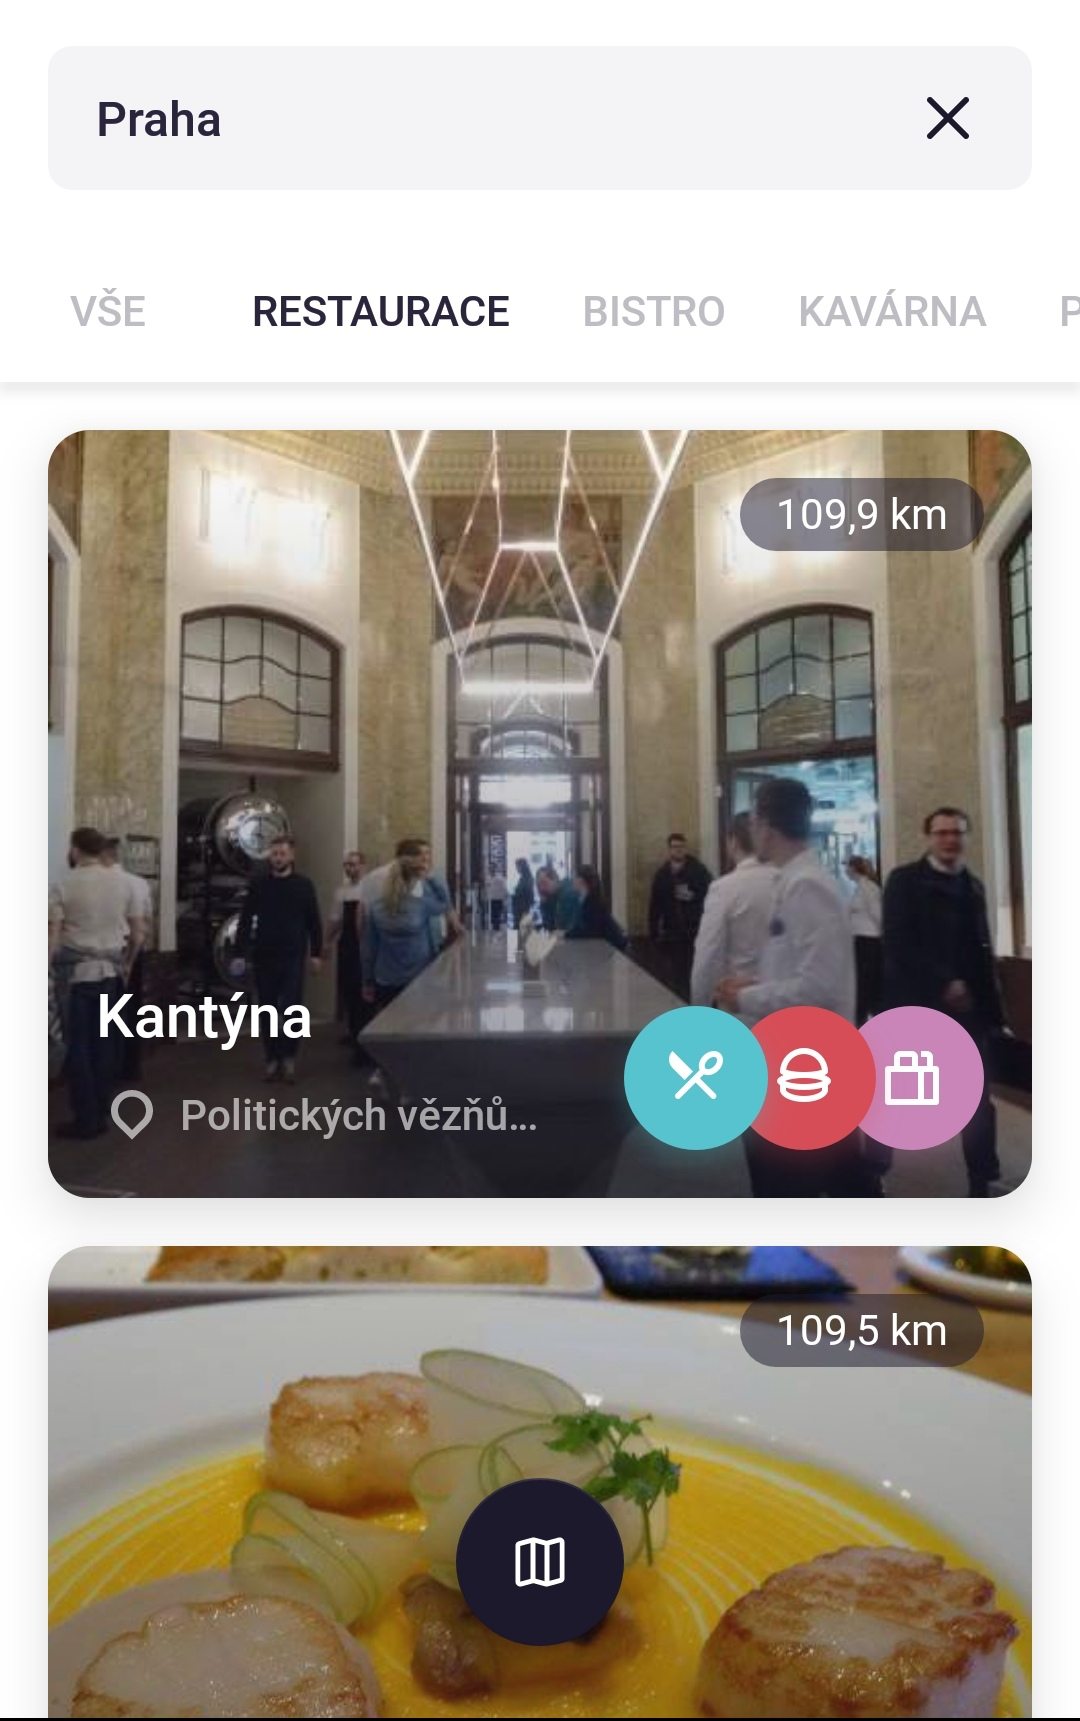
\includegraphics[width=0.33\linewidth]{img/analysis/app-hejlik.jpg}
    \caption{Gastromapa \textit{L. Hejlíka} \cite{app-hejlik}}
    \label{fig:gastromapa-hejlik}
\end{figure}

\subsubsection{The advantages}
\begin{itemize}
    \item Design is fresh, clean and users can immediately see relevant content.
    \item Thanks to clean design application is easy to use and understand.
    \item The whole application behaves smoothly without any noticeable freezing.
\end{itemize}

\subsubsection{The drawbacks}
\begin{itemize}
    \item The navigation button has a blackish colour that after scrolling disappears. If the restaurant has a darker photo, the button is hard to notice. 
    \item When coming back to the main screen, loading of the list is started again, and the previous search is lost.
    \item Detail screen on entry is fully covered with restaurant photo. From a design point of view, it is a nice touch, but users must scroll to see any information. 
\end{itemize}

\subsection{Pivní deník}
Application \textit{Pivní deník} is used to search nearby pubs in the Czech Republic and their beer offer. The content is created by the community, including served beer and their prices.  Application offers searching nearby restaurants filtered by beer brands. Each user can view a history of places they have visited, furthermore they can mark any pub as their favourite and share their experience.


\begin{figure}[ht]
    \centering
    \begin{minipage}{0.45\linewidth}
        \centering
        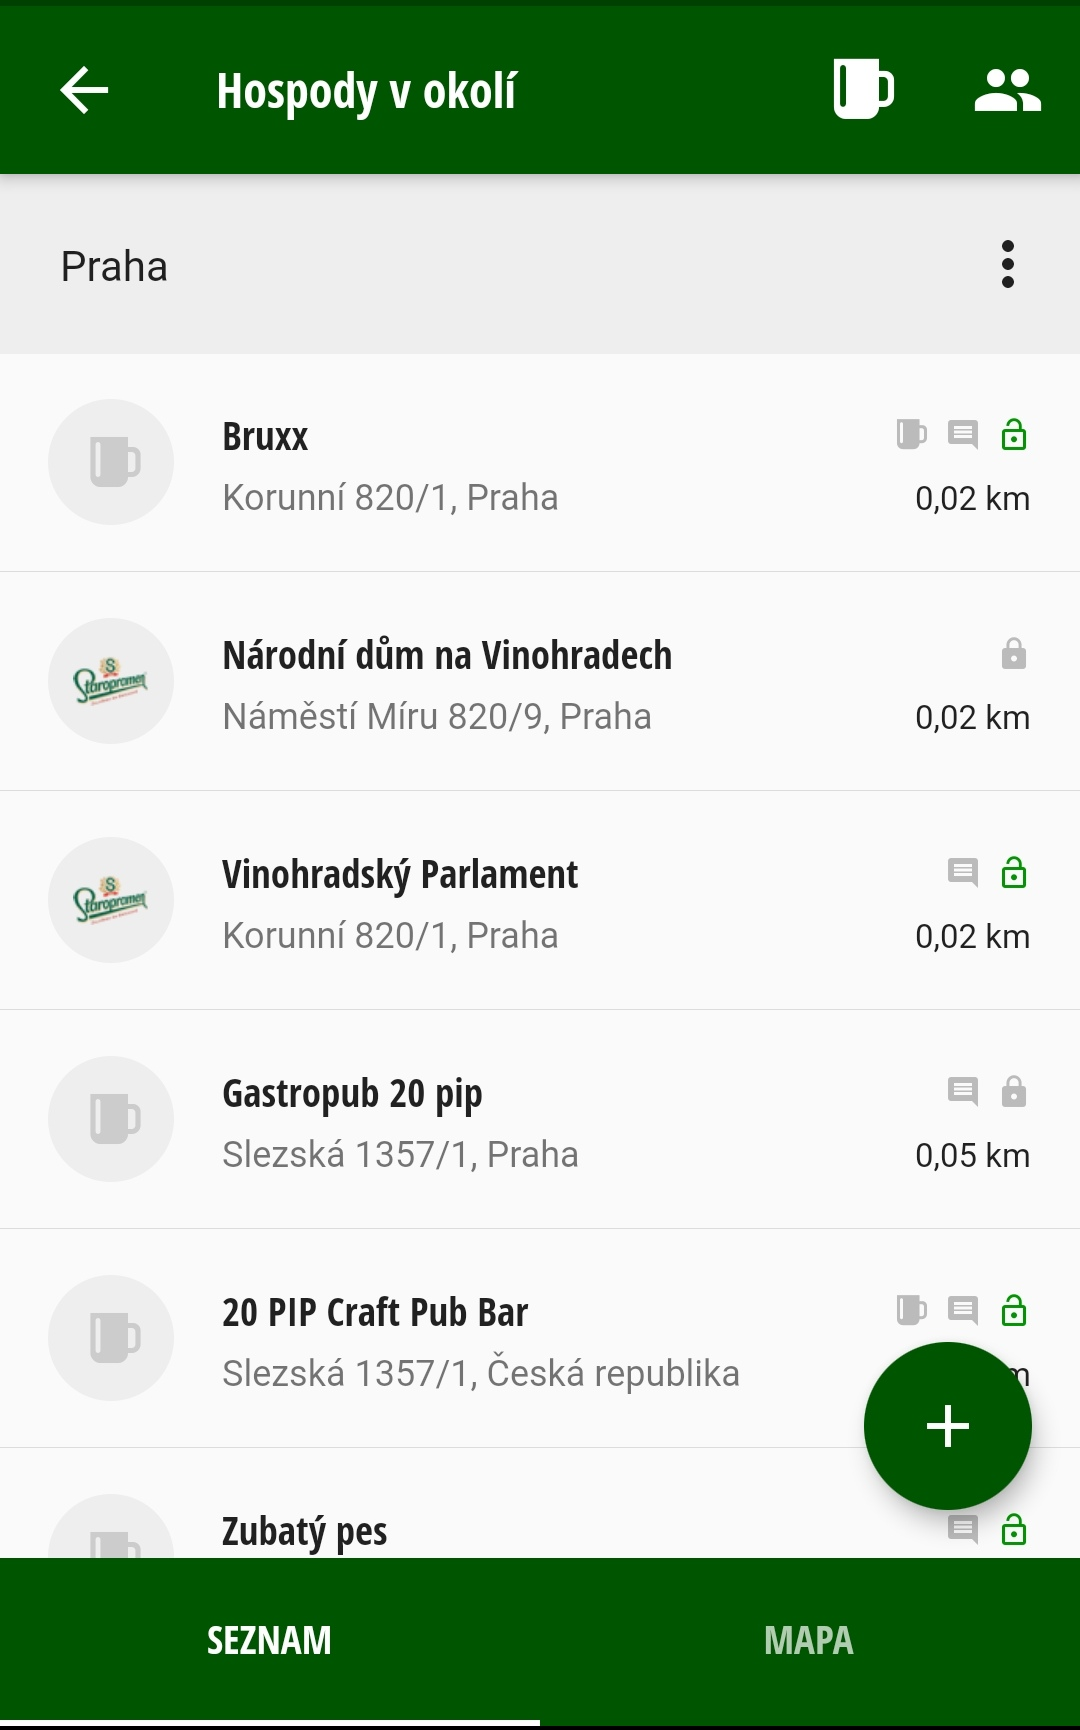
\includegraphics[width=0.75\linewidth]{img/analysis/app-pivni-denik.jpg}
        \caption{Pivní deník \cite{app-pivni-denik}}
        \label{fig:pivni-denik}
    \end{minipage}\hfill
    \begin{minipage}{0.45\linewidth}
        \centering
        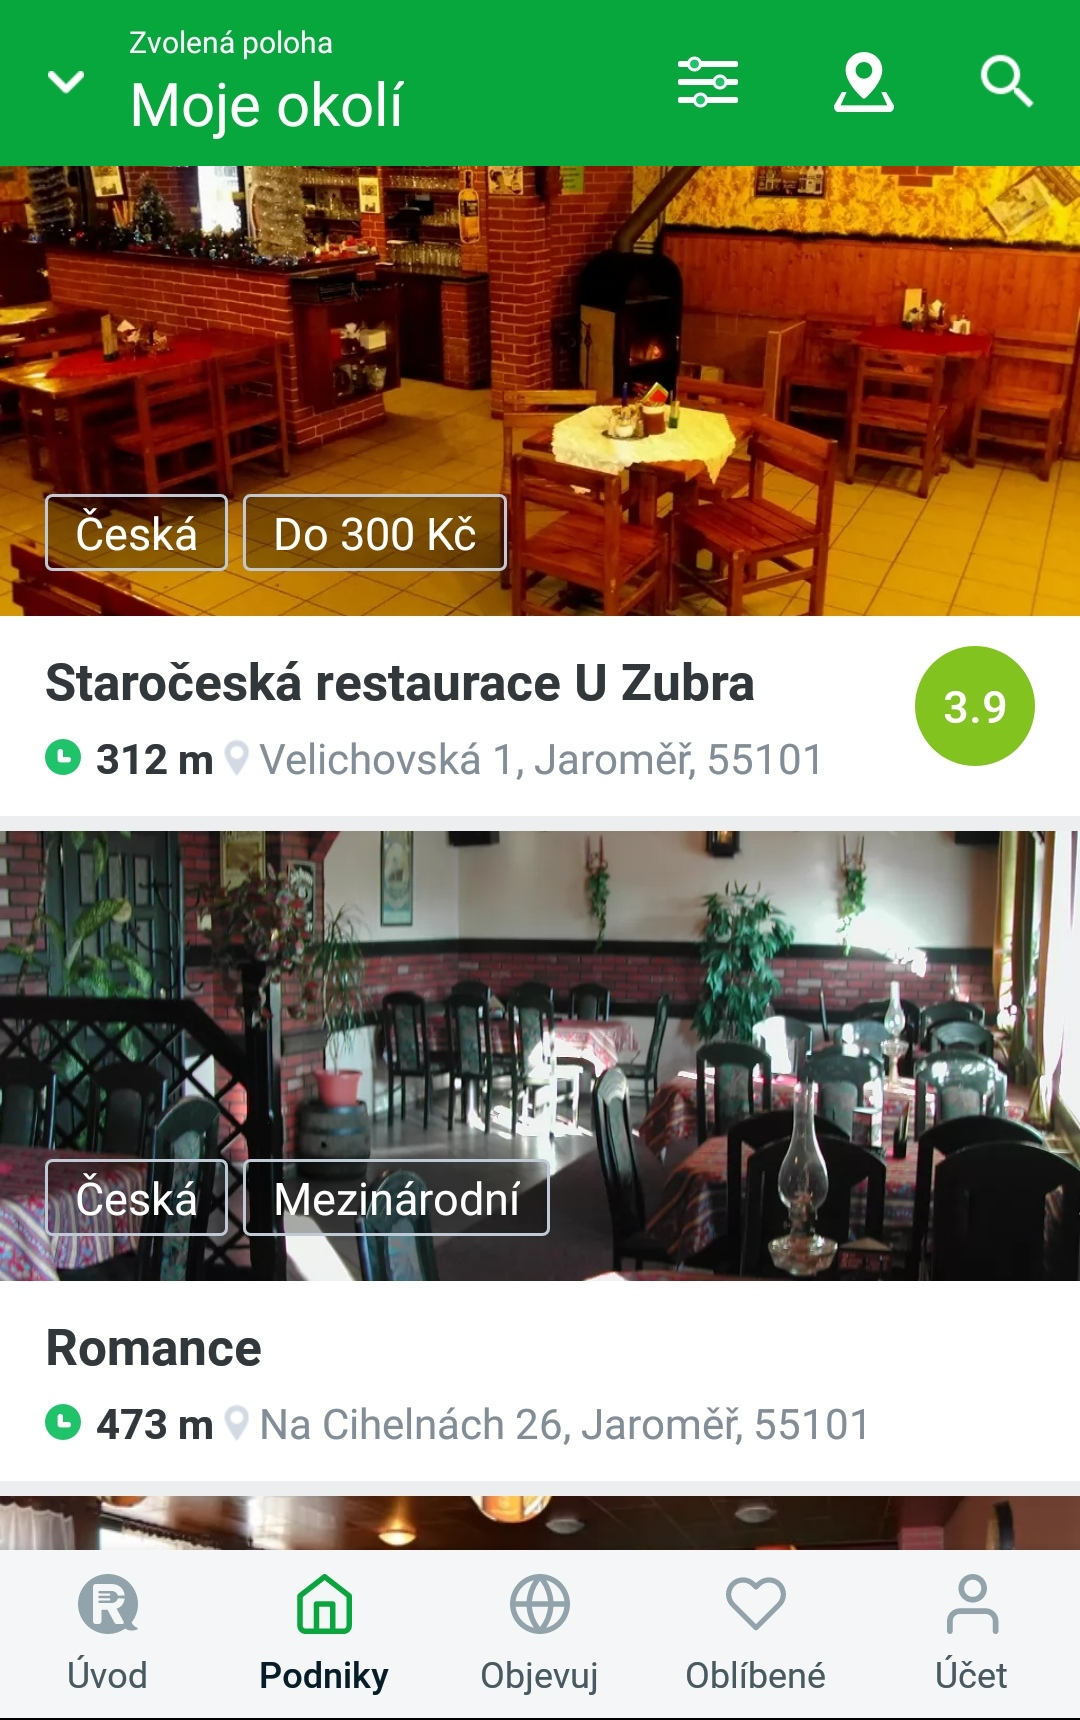
\includegraphics[width=0.75\linewidth]{img/analysis/app-restu.jpg}
        \caption{Restu \cite{app-restu}}
        \label{fig:restu}
    \end{minipage}
\end{figure}

% \begin{figure}[ht]
%     \centering
%     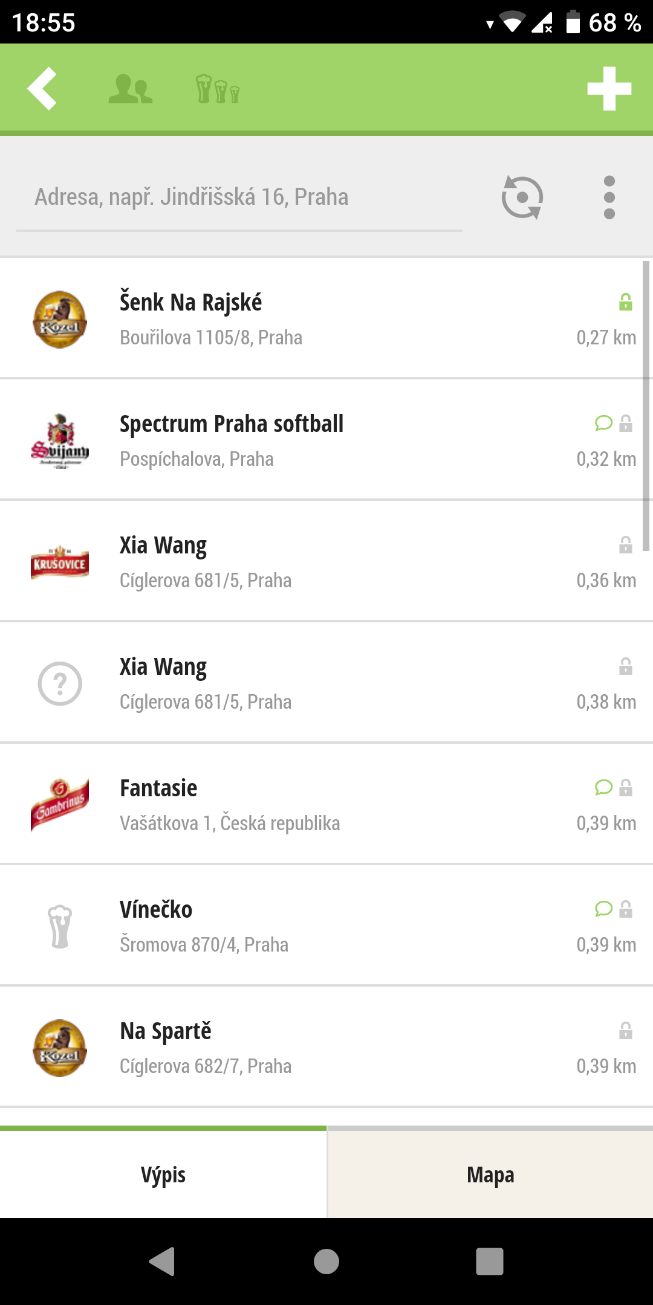
\includegraphics[width=0.25\linewidth]{img/analysis/pivni_denik.png}
%     \caption{Pivní deník \cite{app-pivni-denik}}
%     \label{fig:pivni-denik}
% \end{figure}

\subsubsection{The advantages}
\begin{itemize}
    \item Pubs are displayed as a list or on the map.
    \item The served brands are displayed directly within the list, so it is not needed to visit details.
    \item The registration is optional for searching. If users want to contribute, they have to have an account.
\end{itemize}

\subsubsection{The drawbacks}
\begin{itemize}
    \item Registration can be done through Facebook or e-mail. With e-mail registration, the user is forced to leave the application and is redirected to the web page where registration is finished.
    \item As was said, content is created by the community. During the research, it was clear that many information is outdated or misleading. 
    \item Overall the application design looks outdated and does not meet current, modern,  trends.
    \item On the primary screen there are displayed user's stats and the most three nearest pubs. The~drawback is that on the~larger screens, there is plenty of unused space. 
    \item Each restaurant displays only one brand of drafted beer. Nowadays, many pubs offer more than one brand. 
    \item Side menu can be opened only with the hamburger icon but not with slide to the right gesture.
\end{itemize}

\subsection{Restu}
\textit{Restu} is another gastronomy guide focused on restaurants in the Czech Republic. Through this application reservations can be made. Application has many unique functionalities. For example ``discover'' section which shows attractive offers or the best cafe in the city. Another functionality is the ``check-in'' button which gives credits to the users if they eat at the~given restaurant. Target audience is everyone who searches for new places where to eat and make a~reservation.

% \begin{figure}[ht]
%     \centering
%     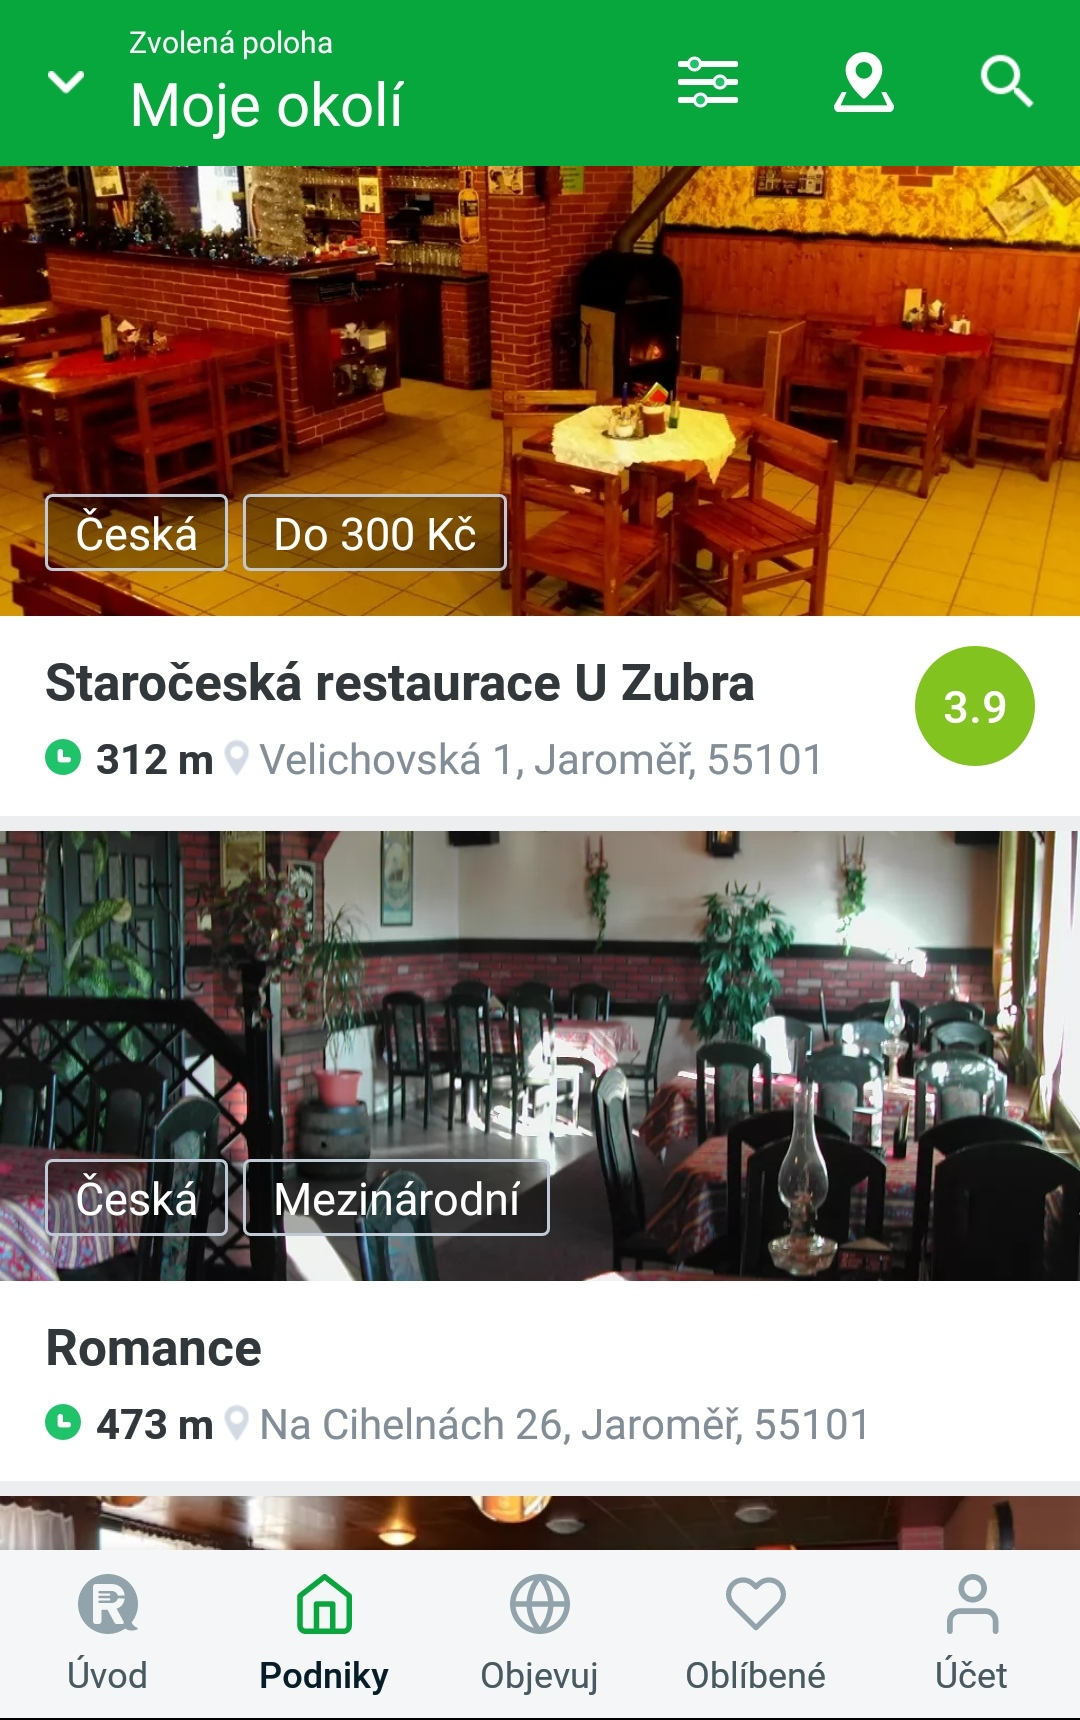
\includegraphics[width=0.33\linewidth]{img/analysis/restu.jpg}
%     \caption{Restu \cite{app-restu}}
%     \label{fig:restu}
% \end{figure}

\subsubsection{The advantages}
\begin{itemize}
    \item Clean and well-structured layout.
    \item Opt-in registration.
\end{itemize}

\subsubsection{The drawbacks}
\begin{itemize}
    \item When a restaurant card is selected, window of the restaurant pops up but at the bottom cannot be hidden again.
    \item To review the restaurant, the user has to be signed in and the restaurant must be open. If the restaurant is closed, the review cannot be added.
\end{itemize}

\subsection{Zomato}
\textit{Zomato} is primarily web-based restaurant browser in the world. It has its own database of establishments. Content is edited by users.  
On the primary screen are displayed ``week hits'', top restaurants or ``happy hours''. Restaurants are divided into categories such as ``Nightlife'' or ``Daily menu'' which helps for navigation within the application.
Target audience is anyone who wants to try new restaurants or someone who is looking for action offers.

% \begin{figure}[ht]
%     \centering
%     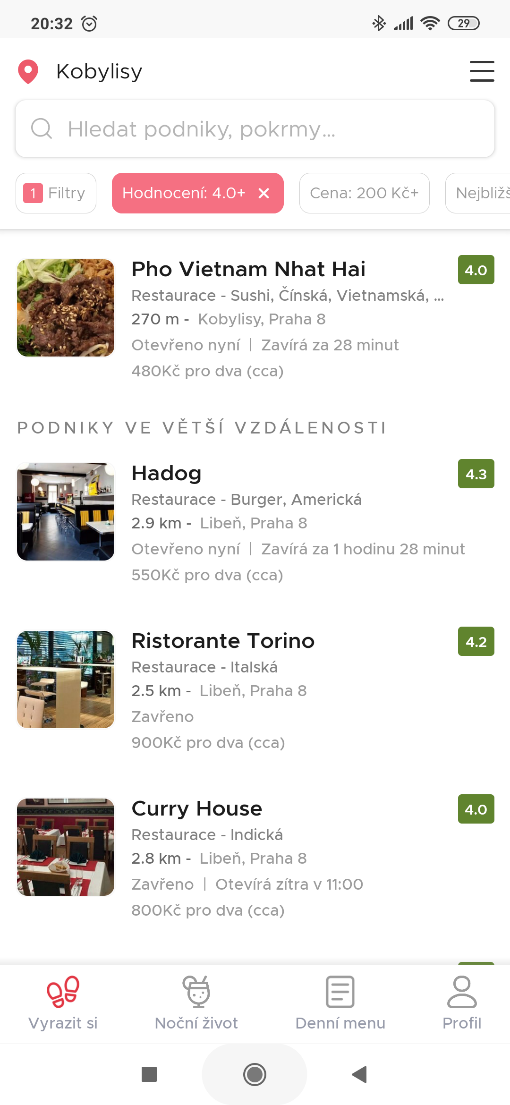
\includegraphics[width=0.33\linewidth]{img/analysis/zomato.png}
%     \caption{Zomato \cite{app-zomato}}
%     \label{fig:zomato}
% \end{figure}

\begin{figure}[ht]
    \centering
    \begin{minipage}{0.45\linewidth}
       \centering
    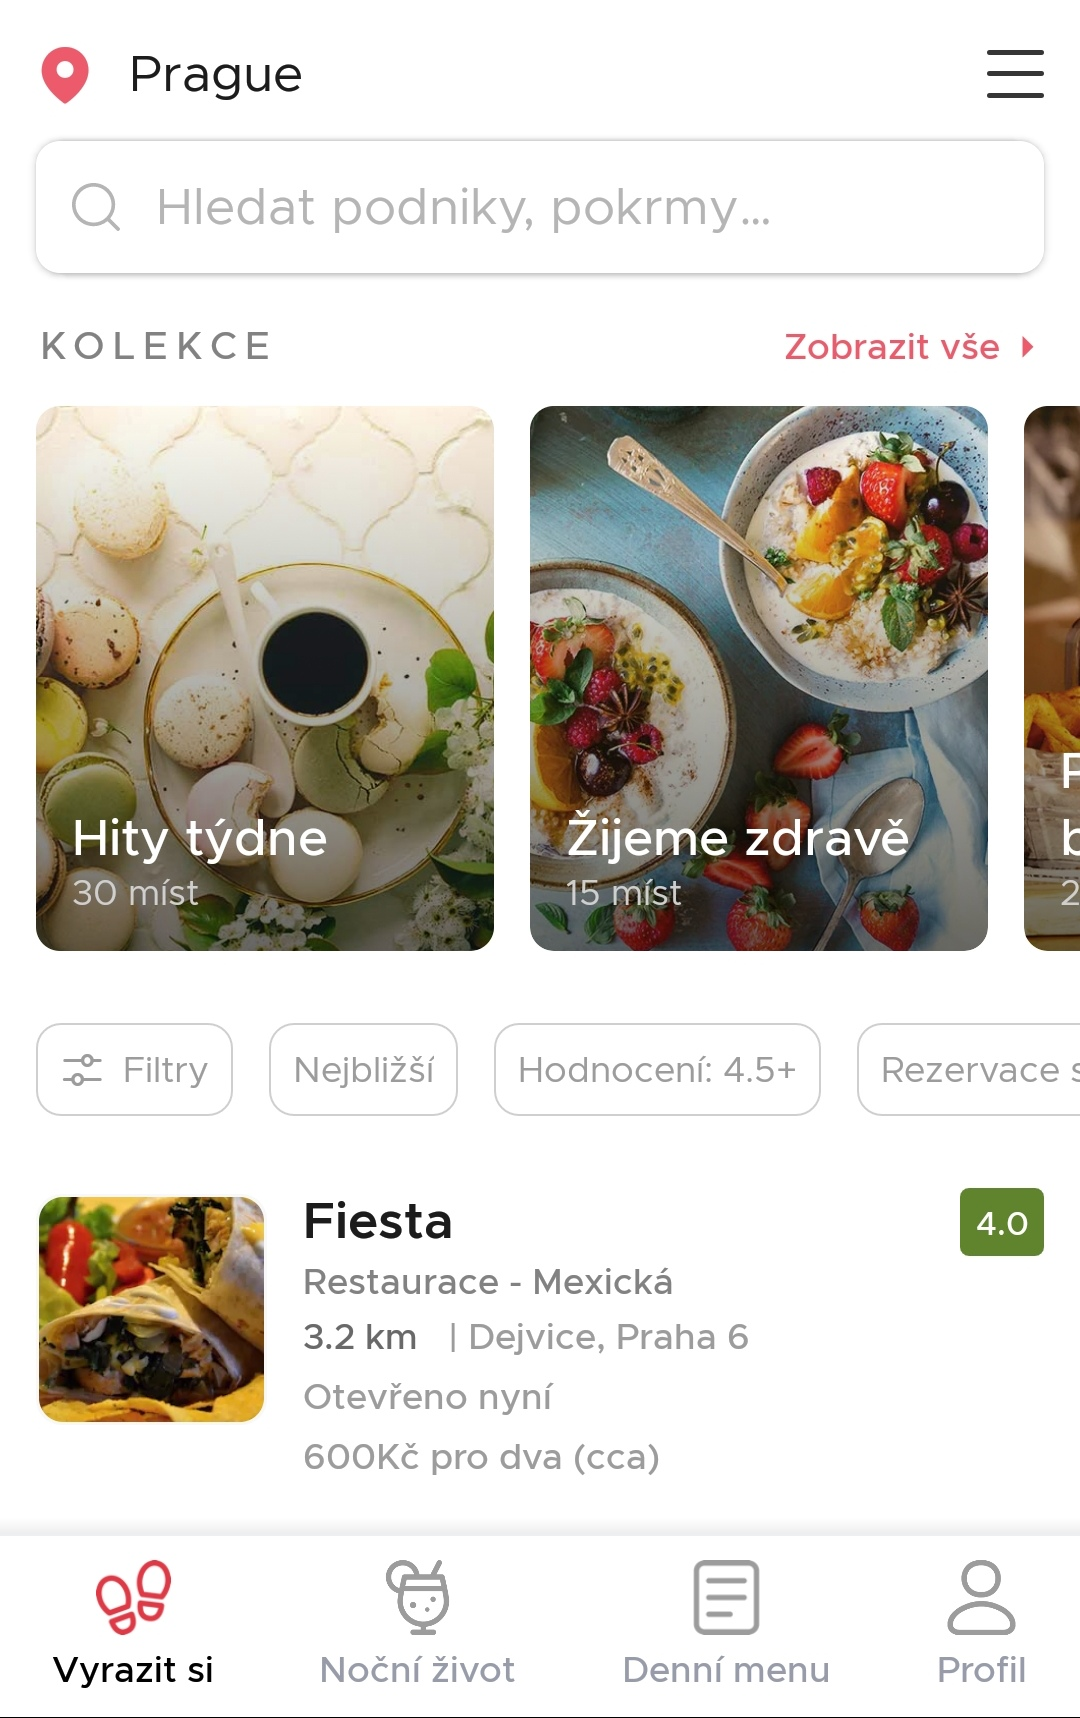
\includegraphics[width=0.75\linewidth]{img/analysis/app-zomato.jpg}
    \caption{Zomato \cite{app-zomato}}
    \label{fig:zomato}
    \end{minipage}\hfill
    \begin{minipage}{0.45\linewidth}
        \centering
        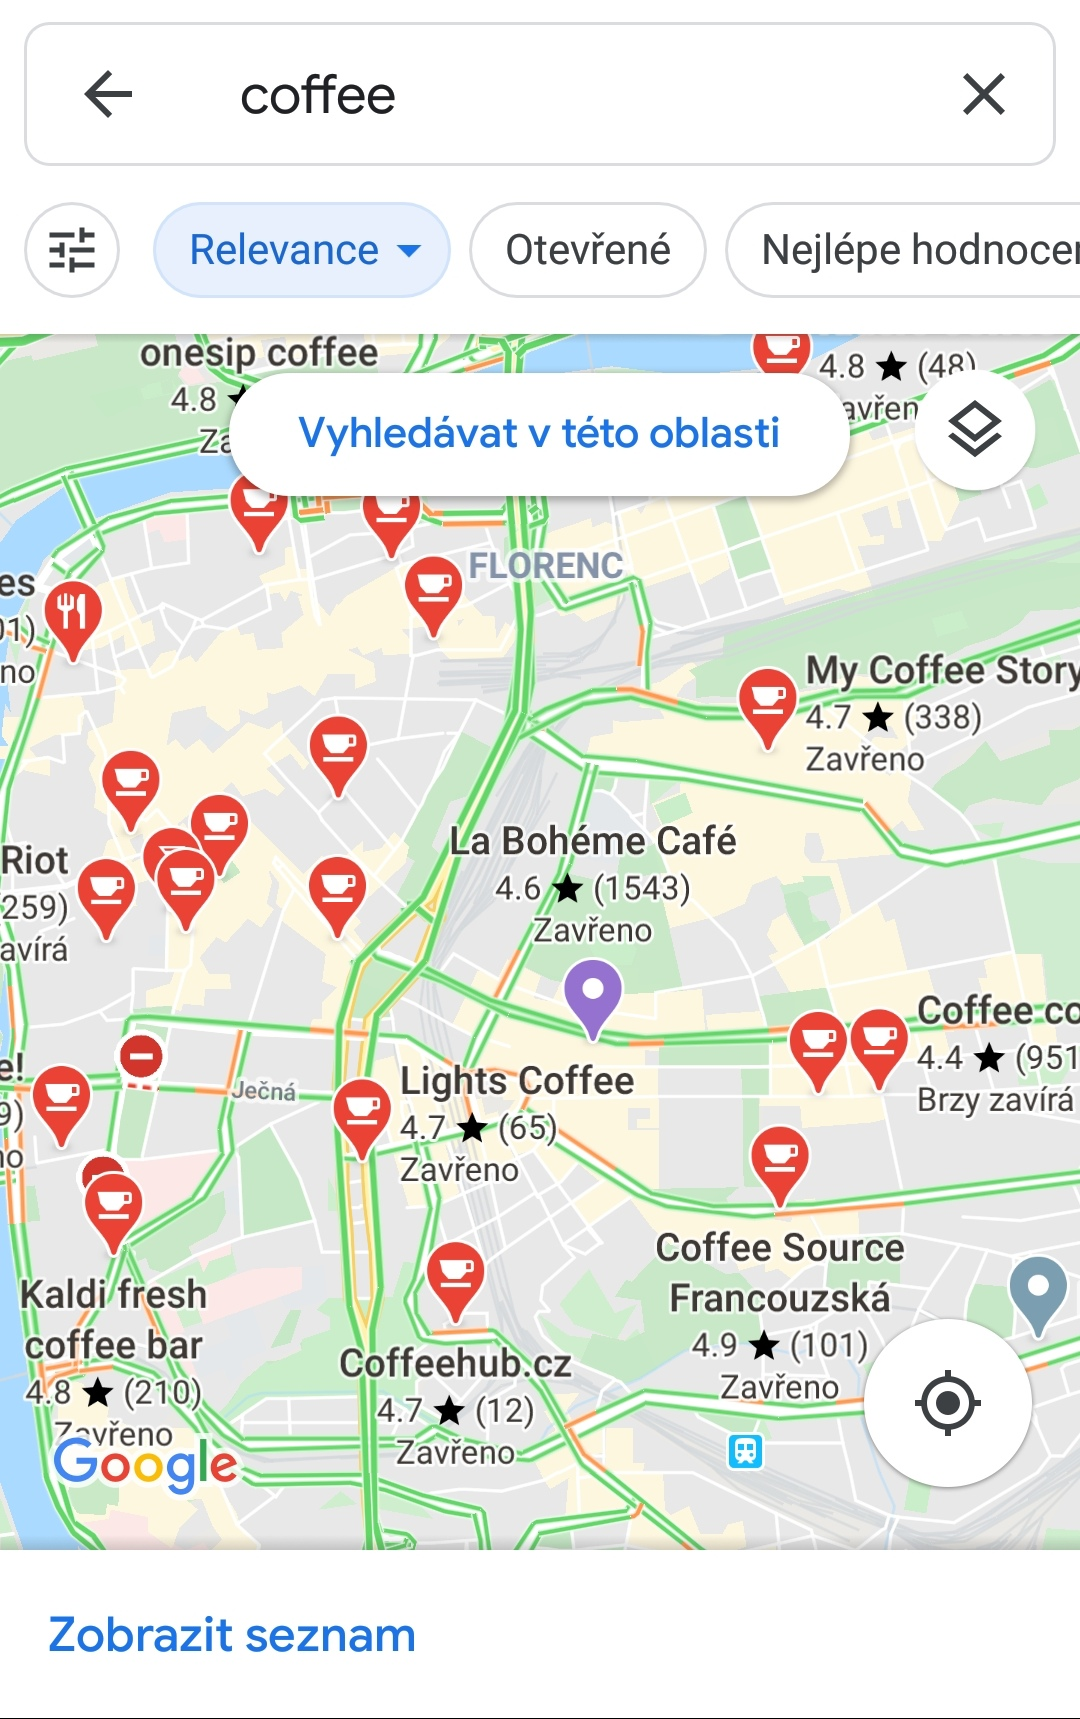
\includegraphics[width=0.75\linewidth]{img/analysis/app-gmaps.jpg}
        \caption{Google Maps \cite{app-google-maps}}
        \label{fig:google-maps}
    \end{minipage}
\end{figure}

\subsubsection{The advantages}
\begin{itemize}
    \item Well solved filtering. Filter setting is intuitive, displays most used filters. 
    \item Advanced options for filtering with tags such as ``dog friendly'' or ``WiFi free''.
    \item Friendships with other users. If another user added a~review, notification is received.
\end{itemize}

\subsubsection{The drawbacks}
\begin{itemize}
    \item The primary screen is cluttered with many information at one place.
    \item Nearby restaurants list is hidden below ``favourites restaurants'' and ``month collections''.
    \item Full-text search in some circumstances behaves unexpectedly. For example, to search for restaurants which offer ``Asian food'' user has to type exactly ``asian'' but not ``asia''.
    \item Readability of some text is worsened by light background and greyish text colour. In some scenarios, it is hard to read.
\end{itemize}

\subsection{Google maps}
Popular worldwide map service by \textit{Google}. One of the world's biggest database of places, restaurants. 
\textit{Google maps} for each business, establishment displays additional info such as user reviews, photos, prices. 
Within Android system is already installed. Nearby places can be searched directly from the map.

% \begin{figure}[ht]
%     \centering
%     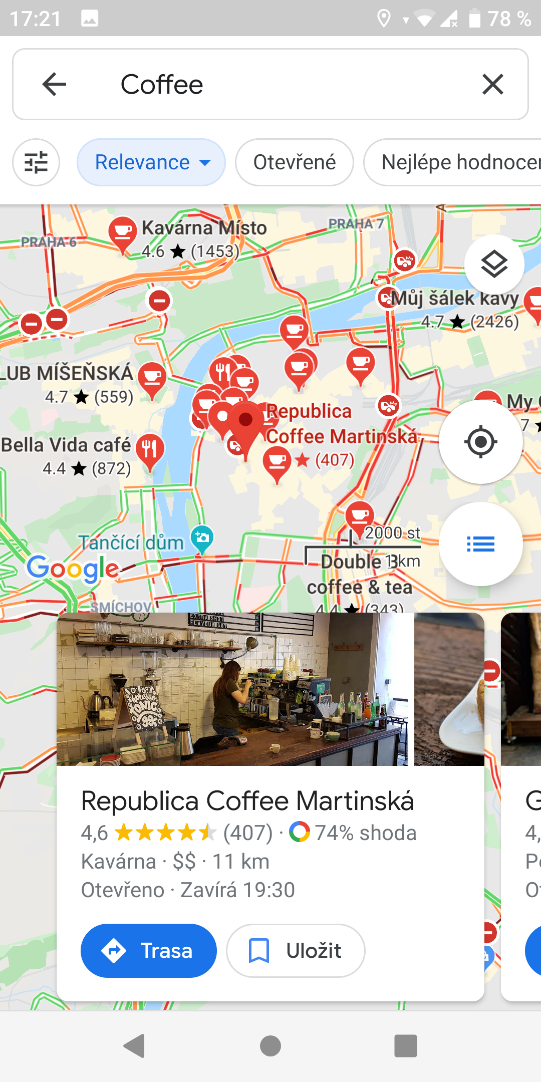
\includegraphics[width=0.33\linewidth]{img/analysis/gmaps.png}
%     \caption{Google Maps \cite{app-google-maps}}
%     \label{fig:google-maps}
% \end{figure}

\subsubsection{The advantages}
\begin{itemize}
    \item Well known and tested user interface which is embedded often to another application.
    \item No registration is required.
    \item Place detail includes plenty of useful information.
    \item GPS navigation with one click.
\end{itemize}

\subsubsection{The drawbacks}
\begin{itemize}
    \item Not domain focused, that means it does not offer focused content on particular businesses such as restaurants.
    \item No advanced filtering and result sorting.
\end{itemize}

In conclusion, five applications were analysed on the Android system. Three apps are focused mainly on gastronomy. Another one specialises on beer. Last one, \textit{Google maps} is one of the most universal and robust. 
Each application has its own unique \gls{ui} and overall user experience differs. In the~\cref{table:app-analysis} the~targeted audience and user interface usefulness is summarised.

\begin{table}[htbp]
\centering
\begin{tabular}{|l|l|l|}
\hline
\multicolumn{1}{|c|}{Application} & \multicolumn{1}{c|}{Targeted audience} & \multicolumn{1}{c|}{Overall \gls{ui}} \\ \hline
Gastromapa Lukáše hejlíka         & Everyone                               & Great                           \\ \hline
Pivní deník                       & Beer drinkers                          & Bad.                            \\ \hline
Restu                             & Everyone                               & Bad.                            \\ \hline
Zomato                            & Everyone                               & Good                            \\ \hline
Google                            & Everyone                               & Great but complex              \\ \hline
\end{tabular}
\caption{Analysed applications \gls{ui} summarization}
\label{table:app-analysis}
\end{table}

% ----- % ----- % ----- % ----- % ----- % ----- % ----- % ----- % ----- % ----- % ----- % ----- % ----- % ----- %
\section{Application prototype}
One crucial step during the creation of software product is prototyping. Prototypes can help introduce different design ideas, can be easily tested, evaluated and changed. Prototyping techniques differ, but the desired output is the same -- provide visually concept of the final product. Prototypes do not help only visually, but they are part of user experience research and can find out which parts of the user interface should be changed before it is implemented.

There is no correct definition of how prototypes should look and how they should be created. The~prototype can be made from the form as a simple sketch on paper to sophisticated pixel-perfect application~\cite{adobe-prototype}. Prototypes can be created multiple times during the whole creation process. 

In the early stages \gls{lofi} prototype is typically created. With \gls{lofi}, the application can be evaluated and user-tested if desired design concept is usable and understandable for users. When \gls{lofi} is finalised, the next prototype~--~\gls{hifi} is created. \gls{hifi} comes out from \gls{lofi} and should behave as fully functional application on the target platform. With \gls{hifi} once again, the application is evaluated with users and tested. 

To be more precise, according to \cite{adobe-prototype} \gls{lofi} prototype, it is a~way to translate high-level concepts into tangible and testable artefacts. The most significant  functionality of \gls{lofi} prototypes is to check and test the functionality of the~product before visual appearance. Advantage of \gls{lofi} is that it is inexpensive, fast way to propose prototype. On the other hand, \gls{lofi} lacks complexity and cannot supply advanced interactivity. \gls{lofi} should be used to quickly create a prototype and get user feedback in the early stages of the creation process. 

After the~\gls{lofi} prototype, the \gls{hifi} is created. This prototype appears and function as similar as possible to the actual built application. \gls{hifi} should be created on the targeted platform and behave as it is the~final product. The goal is to have more complex \gls{ui} interactivity and have better feedback from user testing. Thanks to the fact that prototype looks like a real application user behaves more naturally and can get more precise a meaningful feedback than with \gls{lofi} prototype. 

In conclusion, \gls{lofi} prototypes are tested only internally with a small number of users and can be iterated more often and faster. While \gls{hifi} is more expensive to build and should be created and tested after \gls{lofi} prototype was accepted. On the other hand, \gls{hifi} gives better feedback from user testing, thus provides more valuable information.

\subsection{Coffee Time Prototype}
After the specification was written, next step was to create a \textit{task list}. The task list is written from the user's perspective -- each task describe an user's action. It should tackle all important functionalities and even obvious one such as ``add record'' or ``remove record''.

\begin{figure}[htp]
    \centering
    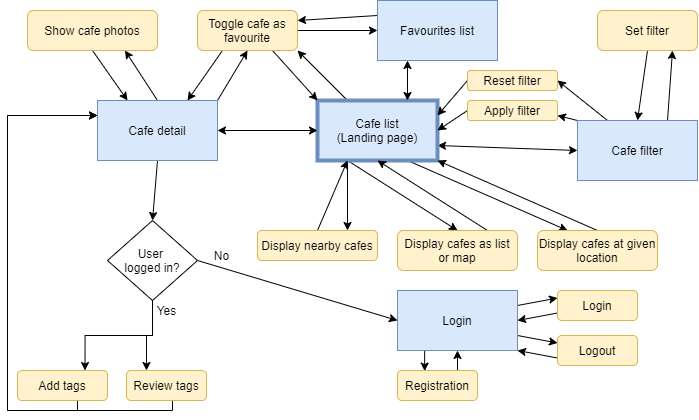
\includegraphics[width=0.9\textwidth]{img/analysis/task-list-graph.png}
    \caption{Coffee Time Task Graph}
    \label{fig:task-graph}
\end{figure}

Because the task list can become very long, it is usually transformed into a \textit{task graph}. The task graph does not have any specific definition, but it should contain every task along with each available screen within the application. Coffee Time's task graph is listed in \cref{fig:task-graph}. The blue rectangles are screens and the yellow ones are any task what users can do. The application's~entry point is highlighted with bold blue rectangle.

A note about \textit{User Interface Design (MI-NUR)} subject which was held during the winter semester of the academic year of 2019/2020. In this subject as a semester work was created the Coffee Time prototype. Sincere gratitude to classmates \textit{Bc. Ondřej John} and \textit{Bc. Vojtěch Polcar} for their co-working on the prototype. Furthermore, much appreciation to \textit{Ing. Jiří Hunka} for feedback and guidance during the work. The classmates helped during prototyping, proposing functionalities, researching and testing. The High-Fidelity prototype was implemented only by the thesis author. 

\subsubsection{Low Fidelity Prototype}
As a task graph was defined, the Lo-Fi prototype could be made. Although the application is considered as multi-platform application, the prototype was focused on Android, and its Material design \cite{material-design}. The inspiration was taken from typical Material layouts, such as AppBar with title and subsequent actions or tabs the bottom of the screen. 

First of all, the rough prototype was drawn on paper. Its purpose was to come up with some ideas and considered layout. After that, the \textit{Balsamiq} \cite{balsamiq} prototyping software was used. The \textit{Balsamiq} tries to mimic pencil and paper. The prototype is created with a set of components which looks like they are drawn by hand.
The most important feature was the ability to create deep links between screens or components. With a few clicks, the prototype was able to handle actions such as the open application menu or navigate to detail. With that tool, the clickable prototype focused on essential app's features was created. As a result, the PDF was exported. The PDF is enclosed as part of the thesis located at \verb|prototype/lofi.pdf|. The portion of the result is shown at \cref{fig:lofi}.

\begin{figure}[htp]
    \centering
    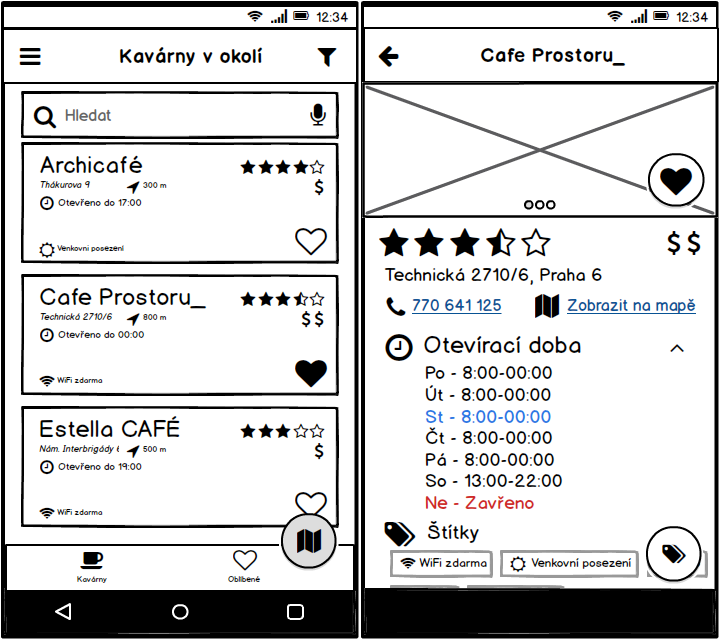
\includegraphics[width=0.75\textwidth]{img/analysis/lofi.png}
    \caption{\gls{lofi} prototype. Cafe list (left) and detail screen (right).}
    \label{fig:lofi}
\end{figure}

The result was tested with co-workers and closest author's family members. From the testing session, useful feedback was given, which is listed along with short answers. 

\begin{questions}
  \item On the cafe list, what if the cafe has more tags than it can display in the row. How to solve it? 
         \begin{answer}
          The solution is to calculate free screen space and display portion of available tags.
         \end{answer}

  \item Research more on how to solve user's reviews.
         \begin{answer}
         As a considered data source is Google Places API, it was acknowledged that it is not possible to add custom reviews through their API.
         \end{answer}
    \item Navigation and contact buttons are too small. 
        \begin{answer}
        Taken into account during implementation.
        \end{answer}
    \item If the tag in detail is clicked, the cafe list with the given tag is shown.
        \begin{answer}
        Taken into account as a valuable tip.
        \end{answer}
    \item Focus on usability with mobile devices, mainly when the user's walk or are in public transport.
        \begin{answer}
        The usability should be more tested. 
        \end{answer}
    \item Focus more to provide understandable information about what tag is and how to use it.
     \begin{answer}
        Information and usability should be more revisited.
    \end{answer}
\end{questions}

\subsubsection{High Fidelity Prototype}
The \gls{hifi} prototype was created as Flutter application. Because of that, in the future, the already written code could be reused. The aim was to create a fully functional prototype for Android devices. As was said earlier in this chapter, the aim of \gls{hifi} is to provide an application so it behaves as real one, which is mainly focused on user interface interaction. That means that the~application does not have any real communication with back-end services. For Coffee Time there was prepared local JSON data source with randomly generated cafe names and their data. Besides that, a few, real one cafes were added to be less general and more known for potential testers. The \gls{hifi} focused on all earlier described use cases. The cafe list screen and cafe's detail screen is shown~at~\cref{fig:hifi}. The prototype's source code can be found at~\verb|https://github.com/petrnymsa/coffee-time/releases/tag/prototype|~\cite{hifi-prototype}. 

\begin{figure}[htp]
    \centering
    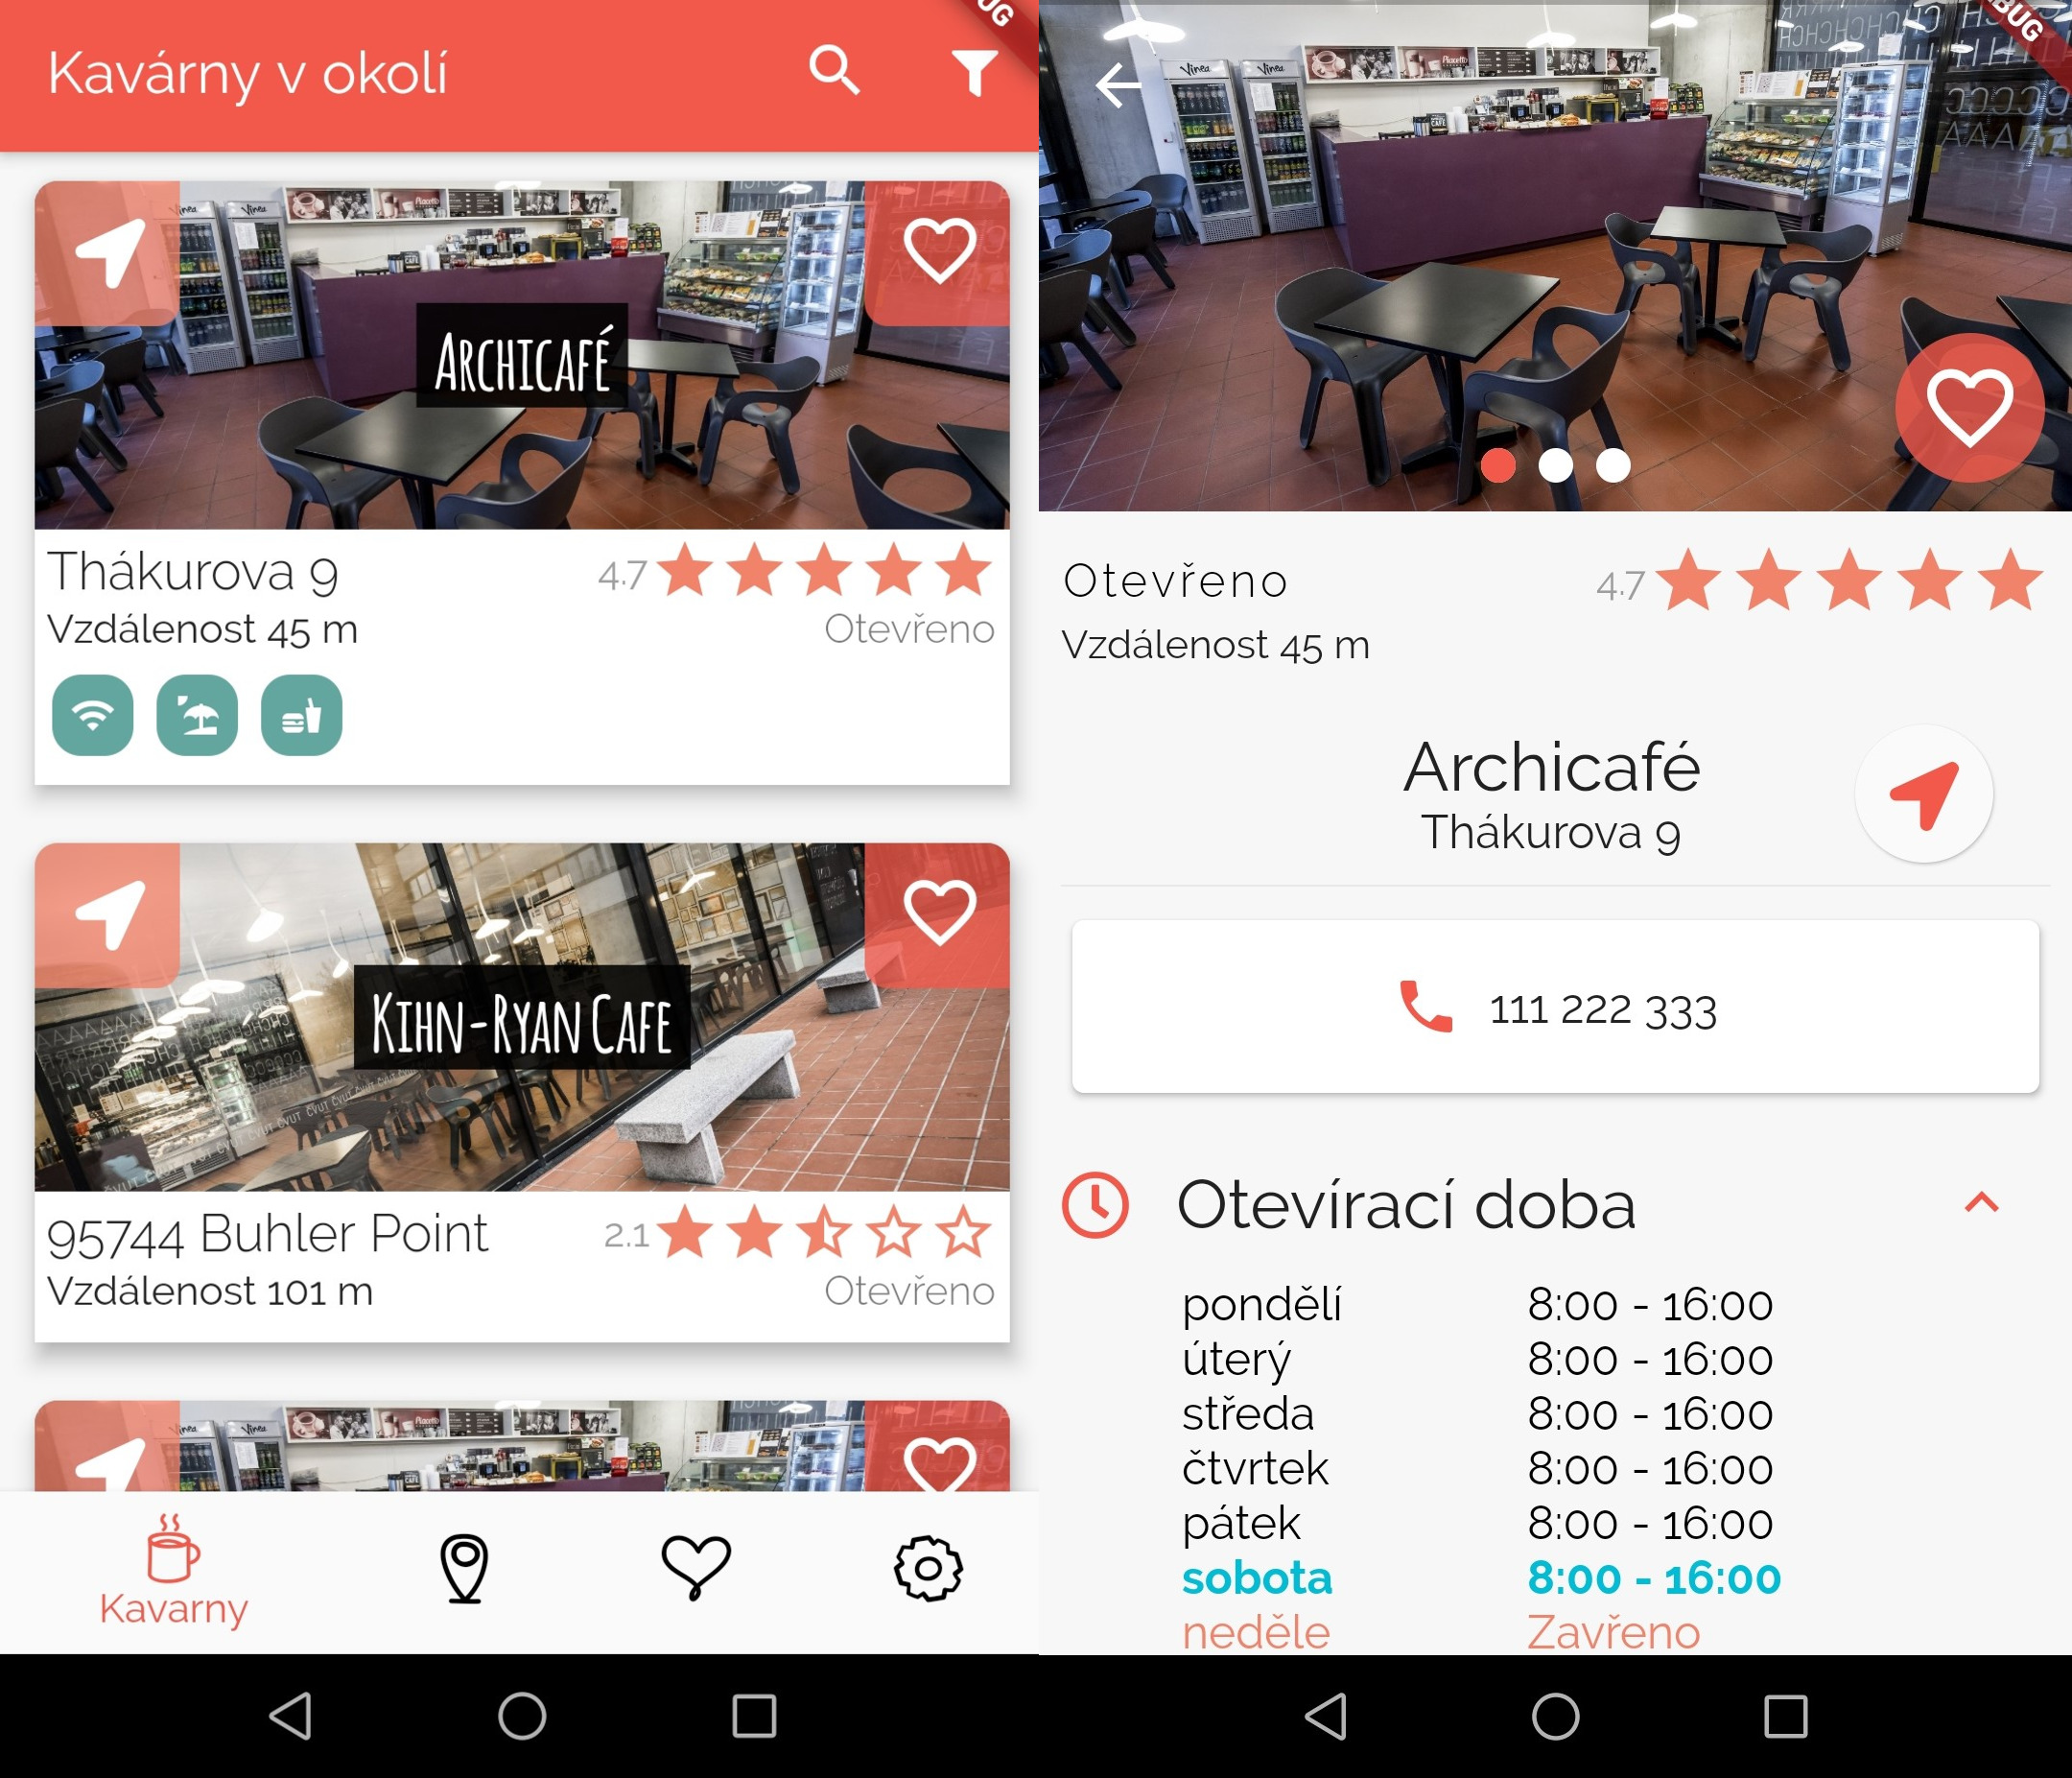
\includegraphics[width=0.6\textwidth]{img/analysis/hifi.jpg}
    \caption{\gls{hifi} prototype. Cafe list (left) and detail screen (right).}
    \label{fig:hifi}
\end{figure}

\subsection{Nielsen Heuristic}
\textit{Nielsen Heuristic}~\cite{nielsen} is a usability engineering method for finding the usability problems in a user interface design so that they can be attended to as part of an iterative design process. Heuristic evaluation involves a small set of rules and these rules should be judged by a small group of ``evaluators''.

Following lines describe one of each of ten rules. Each description is taken from article~\cite{nielsen}.

\begin{enumerate}
    \item \textbf{Visibility of system status} -- The system should always keep users informed about what is going on through appropriate feedback within a reasonable time. 
    
    \item \textbf{Match between system and the real world} -- The system should speak the users' language, with words, phrases and concepts familiar to the user, rather than system-oriented terms. Follow real-world conventions, making information appear in a natural and logical order.
    
    \item \textbf{User control and freedom} -- Users often choose system functions by mistake and will need a clearly marked "emergency exit" to leave the unwanted state without having to go through an extended dialogue. Support undo and redo.
    
    \item \textbf{Consistency and standards} -- Users should not have to wonder whether different words, situations, or actions mean the same thing.
    
    \item \textbf{Error prevention} -- Even better than good error messages is a careful design which prevents a problem from occurring in the first place. Either eliminate error-prone conditions or check for them and present users with a confirmation option before they commit to the action.
    
    \item \textbf{Recognition rather than recall} -- Minimize the user's memory load by making objects, actions, and options visible. The user should not have to remember information from one part of the dialogue to another. Instructions for the use of the system should be visible or easily retrievable whenever appropriate.
    
    \item \textbf{Flexibility and efficiency of use} -- Accelerators — unseen by the novice user — may often speed up the interaction for the expert user such that the system can cater to both inexperienced and experienced users. Allow users to tailor frequent actions.
    
    \item \textbf{Aesthetic and minimalist design} -- Dialogues should not contain information which is irrelevant or rarely needed. Every extra unit of information in a dialogue competes with the relevant units of information and diminishes their relative visibility.
    
    \item \textbf{Help users recognise, diagnose, and recover from errors} -- Error messages should be expressed in plain language (no codes), precisely indicate the problem, and constructively suggest a solution.
    
    \item \textbf{Help and documentation} -- Even though it is better if the system can be used without documentation, it may be necessary to provide help and documentation. Any such information should be easy to search, focused on the user's task, list concrete steps to be carried out, and not be too large.
\end{enumerate}

\subsubsection{Coffee Time Evaluation}
During \textit{MI-NUR} lecture, the above-described heuristic was evaluated against \gls{hifi} prototype. Each screen was taken individually and judged with all rules. Note that only found rules violation are described for each screen.

\begin{itemize}
    \item Cafe list
    \begin{itemize}
        \item Rule \#2: Some tags icons are hard to understand, and their meaning can be easily misunderstood. 
        \item Rule \#8: When filtering is on, it occupies nearly one-third of the screen.
        \item Rule \#9: There is no visible error handling for missing internet connection or location services.
    \end{itemize}
    \item Favourites cafes
    \begin{itemize}
        \item Rule \#2: Same as Cafe list.
        \item Rule \#3: When a favourite cafe is set off, there is no indication that action is permanent without the ability to undoing it. 
    \end{itemize}
    \item Detail screen
    \begin{itemize}
        \item Rule \#2: Same as Cafe list.
        \item Rule \#6: It is not clear how to start navigation. This functionality is provided by the button to the right of the cafe's address. There should be a more visible indication that this action is possible.
    \end{itemize}
    \item Map  screen -- No rules violation found. 
    \item Filter screen -- The only violation is the same as within Cafe list about icons.
\end{itemize}

Once the violations are found, they should be prioritised. The priority indicates how serious violation is. The more severe violation, the more unusable is it for users. The priorities are 

\begin{itemize}
    \item 1 -- negligible
    \item 2 -- visible issue
    \item 3 -- the usability can suffer
    \item 4 -- frustrating experience
    \item 5 -- User is not able to use application at all
\end{itemize}

The most violated rule is number \#2 with tag icons. With this issue suffer most of the screen, because icons are used very often.  This issue has priority 3.  The second issue with favourites cafes (priority 2) can be solved, for example, with small notification with the undo button. The prototype does not have implemented any kind of error handling regarding internet connection or location services (priority 2). 

\subsection{User Testing}
The prototype was tested with seven testers. An important note is that four testers are people who have ``IT knowledge'' and are classmates from university. It was assumed that their understanding could vary against other testers.

The process of testing was as follows -- application was launched on a real device. Each testing was recorded. The recording was essential to know what testers thought, how they used the application and behaved. Each user had the same set of use case scenarios, and the supervisor did not interact either provide any advice to testers how to proceed. There was only one exception when the supervisor was allowed to advise, and that was when tester did not know how to proceed -- he became ``totally lost''. This situation could indicate two different things. First, from the test case scenario, it was not particularly evident what tester should do. Secondly, the test case was understandable, but the application interface not. The second problem is more important for testing and the results.  The test case scenario can be rewritten or with the help of supervisor fully explained. 

The description of test case scenarios, along with established issues, follows. Each test case has an introduction for users in which situation they are.  Next contains test case goal, expected user behaviour and actual behaviour. Note that, the actual behaviour is not part of this summarization. Instead, the~found issues are summarised. 

\subsubsection{Test Case 1: Favourite Cafe}
User visits his favourite cafe and he would like to add this Cafe to his favourite list. 
\begin{itemize}
    \item \textbf{Goal} -- Add Cafe to favourites.
    \item \textbf{Expected behaviour}
    \begin{enumerate}
        \item User is located on the cafe list screen. The targeted cafe is displayed.
        \item User clicks on the heart icon located in top right corner of the cafe's tile. 
        \item Alternative flow: User is located on detail screen and taps heart icon located on the top of the screen. 
    \end{enumerate}
    \item \textbf{Found Issues} -- The testers went through a test case without any issues.
\end{itemize}

\subsubsection{Test Case 2: Start Navigation to Selected Cafe}
User has selected cafe and wants to navigation to the cafe's location.
\begin{itemize}
    \item \textbf{Goal} -- Start navigation.
    \item \textbf{Expected behaviour}
    \begin{enumerate}
        \item User is located on the cafe list screen. The targeted cafe is displayed.
        \item User clicks on the navigation icon located in top left corner of the cafe's tile. 
        \item Alternative flow: User is located on the detail screen and taps navigation icon located to the right of address.
    \end{enumerate}
    \item \textbf{Found Issues}
    \begin{enumerate}
        \item Three different icons used to start navigation. Icon is different on the cafe list from icon within detail screen.
        \item In the detail screen, it is not clear that icon can start navigation.
    \end{enumerate}
    \item \textbf{Proposed solution}
    \begin{enumerate}
        \item Use same icon everywhere.
        \item The same problem stated in the Nielsen heuristic evaluation. The icon should be highlighted. Can be added ``elevation''~\cite{material-design-elevation} -- shadow under the component to provide depth. 
    \end{enumerate}
\end{itemize}

\subsubsection{Test Case 3: Filter Cafes with Tags}
User is interested in cafes where they offer beside the coffee has also beer.
\begin{itemize}
    \item \textbf{Goal} -- Filter Cafes that has ``beer'' tag.
    \item \textbf{Expected behaviour}
    \begin{enumerate}
        \item On the cafe list screen, the user selects filter icon to open filter screen.
        \item Within filter screen, the user selects to filter by tags and choose ``beer''.
        \item User confirms the filter. 
    \end{enumerate}
    \item \textbf{Found Issues}
    \begin{enumerate}
        \item ``Filter screen is confusing. Confirmation is useless.''
        \item ``Do not open filter screen, just open some modal window to selects tags''.
        \item The filter icon is unclear.
        \item ``If the user is located on the detail screen, clicking on the tag icon should set the~ filter.'' 
    \end{enumerate}
    \item \textbf{Proposed solution}
    \begin{enumerate}
        \item The filter icon is standardised icon. 
        \item Clicking on tag should set the filter. 
    \end{enumerate}
\end{itemize}

\subsubsection{Test Case 4: Suggest New Tag}
User visits regularly cafe which is friendly to dog owners. The user found out that this information is missing in the application. 
\begin{itemize}
    \item \textbf{Goal} -- The user suggests tag ``dog friendly'' or similar for the cafe. 
    \item \textbf{Expected behaviour}
    \begin{enumerate}
        \item User selects cafe and opens detail screen.
        \item User clicks on ``suggest change''.
        \item User adds tag ``dog friendly'' and confirms suggestion.
    \end{enumerate}
    \item \textbf{Found Issues} -- No issues found.
\end{itemize}

\subsubsection{Test Case 5: Tag review}
User visits regularly cafe which has mistaken information about ``available parking''. He would like to inform about this wrong tag. 
\begin{itemize}
    \item \textbf{Goal} -- The user should review ``parking'' with dislike. 
    \item \textbf{Expected behaviour}
    \begin{enumerate}
        \item User selects cafe and opens detail screen.
        \item User clicks on ``suggest change''.
        \item User reviews ``parking'' with dislikes and confirms suggestion. 
    \end{enumerate}
    \item \textbf{Found Issues} -- No issues found.
\end{itemize}

\subsubsection{Test Case 6: Most popular nearby cafe}
User wants find the most popular cafe around him. 
\begin{itemize}
    \item \textbf{Goal} -- The user change ordering from ``by distance'' to ``by popularity''.
    \item \textbf{Expected behaviour}
    \begin{enumerate}
        \item User opens filter screen.
        \item User changes to ordering by popularity.
        \item User confirms filter.
    \end{enumerate}
    \item \textbf{Found Issues} -- No issues found.
\end{itemize}

From testers was obtained beneficial feedback which helps to tune user interface for better usability. Besides feedback from individual test cases, a few additional tips were given.

\begin{itemize}
    \item Cafe's name on tile can be harder to read with the contrasting background image. \textit{Can be solved with making photo darker.}
    \item Landscape mode is not working. \textit{During prototype it wasn't considered.}
    \item The map marker could contain more information than cafe's name.
\end{itemize}

All feedback was gathered and was taken into account during the next phase of implementation.
% ----- % ----- % ----- % ----- % ----- % ----- % ----- % ----- % ----- % ----- % ----- % ----- % ----- % ----- %
\section{Back-end Analysis}
In this section, the technical analysis of available technologies for back-end services is discussed. The focus is only on the back-end part. The technical detail of the mobile application is discussed in the next~\cref{ch:implementation}.

One vital part of the whole architecture is~\gls{gpa}~\cite{google-places-api}. This API offers access to Google Maps services, searching places, place details, place photos and more. The API has five services~\cite{google-places-api}. 

\begin{itemize}
    \item Place search -- a list of places based on the user's location or search query.
    \item Place details -- returns more detail information about a specific place.
    \item Place photos -- provides access to place-related photos.
    \item Place autocomplete -- automatically fills in the name or address of a place.
    \item Query autocomplete -- provides a query prediction service for text-based geographic searches.
\end{itemize}

To access these services, the Google~API~Key must be obtained~\cite{google-places-api-key}.
% --- # --- # --- # --- # --- # --- # --- # --- # --- # --- # --- # --- # --- # --- # --- # --- # --- # --- #
\subsection{Google Places API}
The Google Places API returns plenty of information about each place, but the application uses an only subset of available information. The application makes usage of four available services - Find a place, Nearby search, Place detail and Place photos. Some parameters are the same for each service, and the output of each service is similar. 

Each place has several fields such as name, address, location, rating and much more. However, not every field is used in the application, and it is not necessary to obtain these fields in the response. On top of that, each field is included in the pricing category. That means that some of the fields are more expensive to obtain than others~\cite{google-places-api-billing}. It was important to analyse which fields are essential to get before the API model could be created. Following lines summarize each API usage, its parameters, fields and expected output.
% --- & --- & --- & --- & --- & --- & --- & --- & --- & --- & --- & --- & --- & --- & --- & --- & --- & --- &
\subsubsection{Find Place}
The purpose of this service is to find places based on the text-based query or custom location.  \Cref{table:gapi-find-place-params} describes each of used parameter.\Cref{table:gapi-find-place-fields} describes each expected field in the response. 

\begin{table}[htbp]
\centering
\begin{tabularx}{\textwidth}{|l|X|}
\hline
\textbf{Parameter} & \textbf{Usage}                                                    \\ \hline
key                & API key                                                           \\ \hline
input              & search query                                                      \\ \hline
inputtype          & set to textquery                                                  \\ \hline
language           & language code                    \\ \hline
locationbias       & set to circle:radius@lat,lng.                                     \\ \hline
\end{tabularx}
\caption{Find place parameters}
\label{table:gapi-find-place-params}
\end{table}
% ------
\begin{table}[htbp]
\centering
\begin{tabularx}{\textwidth}{|l|X|}
\hline
\textbf{Field}     & \textbf{Description}                                                      \\ \hline
place\_id          & unique place identification                                                \\ \hline
name               & place's name                                                              \\ \hline
icon               & place's icon                                                              \\ \hline
geometry           & geolocated latitude,longitude                                             \\ \hline
formatted\_address & human-readable address                                                    \\ \hline
types              & list of place categories such as ``cafe''                                 \\ \hline
photos             & contains photo width, height and photo\_reference                          \\ \hline
opening\_hours     & contains only open\_now. For full information, detail request is required \\ \hline
price\_level       & value from 0 to 4                                                         \\ \hline
rating             & value from 1.0 to 5.0                                                     \\ \hline
\end{tabularx}
\caption{Find place fields}
\label{table:gapi-find-place-fields}
\end{table}
% --- & --- & --- & --- & --- & --- & --- & --- & --- & --- & --- & --- & --- & --- & --- & --- & --- & --- &
\subsubsection{Nearby Search}
\textit{Nearby Search} allows finding nearby places around the given location. In contrast with \textit{Find place}, the \textit{Nearby Search} returns all fields available to place and can return up to~60~places. The result is paginated~up~to three pages with~20~places in each page. If the result has another page, the pagetoken is included in the response. As before the \cref{table:gapi-nearby-search-parameters} shows service parameters.

\begin{table}[htbp]
\centering
\begin{tabularx}{\textwidth}{|l|X|}
\hline
\textbf{Parameter} & \textbf{Usage} \\ \hline
key                & API key \\ \hline
location           & latitude,longtitude \\ \hline
radius             & circular radius in meters, max 50 000m  \\ \hline
language           & language code \\ \hline
opennow         & place should be open. If place does not have this field, it is omitted from results  \\ \hline
type & place type, always set to \textit{cafe} \\ \hline
pagetoken & token for next page \\ \hline 
\end{tabularx}
\caption{Nearby Search parameters}
\label{table:gapi-nearby-search-parameters}
\end{table}
% --- & --- & --- & --- & --- & --- & --- & --- & --- & --- & --- & --- & --- & --- & --- & --- & --- & --- &
\subsubsection{Place Details}
Each place has additional information accessible through place details. \Cref{table:gapi-details-parameters} describes each parameter used, and~\cref{table:gapi-find-place-fields} describes fields which should be returned in the response.

\begin{table}[htbp]
\centering
\begin{tabularx}{\textwidth}{|l|X|}
\hline
\textbf{Parameter} & \textbf{Usage} \\ \hline
key                & API key \\ \hline
place\_id           & place's id \\ \hline
language           & language code \\ \hline
\end{tabularx}
\caption{Place Details parameters}
\label{table:gapi-details-parameters}
\end{table}

\begin{table}[htbp]
\centering
\begin{tabularx}{\textwidth}{|l|X|}
\hline
\textbf{Parameter} & \textbf{Usage} \\ \hline
international\_phone\_number           & phone number in international format \\ \hline
opening\_hours           & opening times and if is currently open \\ \hline
photos                & additional up to ten photos \\ \hline
review           & up to five user reviews \\ \hline
utc\_offset           &  offset in minutes from UTC \\ \hline
website           & place's website \\ \hline
\end{tabularx}
\caption{Place Details fields}
\label{table:gapi-details-fields}
\end{table}

Note that \textit{opening\_hours} contains localised \textit{weekday\_text}. If a place is always open, the \textit{close} field within \textit{opening\_hours} is missing and \textit{open} field has day equal to zero and time equal to ``0000''.
% --- & --- & --- & --- & --- & --- & --- & --- & --- & --- & --- & --- & --- & --- & --- & --- & --- & --- &
\subsubsection{The API Response Format}
The \gls{gpa} can respond with \textit{JSON} or \textit{XML} format. The \textit{JSON} format was chosen as a~more typically used and standard format for REST~API and mobile communication~\cite{xml-vs-json}. 

\begin{listing}[h!]
\begin{minted}{json}
{
  "html_attributions": [],
   "results": [      
      {
         "business_status": "OPERATIONAL",
         "id": "0c19db184d6705e945686f3d83ae02a3fbf23068",
         "name": "JS Café",
         "opening_hours": {
            "open_now": true
         },
      }
   ],
   "status": "OK"
}
\end{minted}
\caption{Nearby Search example output (shortened).}
\label{listing:gapi-example-response}
\end{listing}

The \textit{Find Place}, \textit{Nearby Search} and \textit{Place Details} has similar response format where \verb|<status>| indicates response code because \gls{gpa} for every request always responds with HTTP status code 200~OK. The status field can have several values such as \verb|OK| for successful request, \verb|ZERO_RESULTS| for empty results or \verb|INVALID_REQUEST| for general invalid request. Each service has different result field name -- \verb|candidates| for \textit{Find Place}, \verb|results| for \textit{Nearby Search} and~\verb|result| for \textit{Place Details}. An~example output is shown~at~\cref{listing:gapi-example-response}.
% --- & --- & --- & --- & --- & --- & --- & --- & --- & --- & --- & --- & --- & --- & --- & --- & --- & --- &
\subsubsection{Place Photos}
Each place can have photos. The response from \textit{Find Place} or \textit{Nearby Search} contains \verb|photo_reference| along with width and height of the photo. For~obtaining actual photo itself, the~ \textit{Place Photos} endpoint must be called. The~endpoint accepts as always the \verb|key| (API key) and \verb|photo_reference|. The~result can be altered with parameters for maximal width or height. Returns byte encoded image if the request was successful otherwise HTTP status code ``\textit{400 Bad Request}'' or ``\textit{403 Forbidden}'' if the quota limit was reached. 

Although Google Places API returns plenty of information about each place, one added benefit of the Coffee Time application is user suggested tags. This requirement cannot be fulfilled only with Places API, so there is a requirement for another, custom, API. 
% --- # --- # --- # --- # --- # --- # --- # --- # --- # --- # --- # --- # --- # --- # --- # --- # --- # --- #
\subsection{Coffee Time API}
The~\gls{cta} will be used for two main functionalities. First of all, it will provide access to Google Places API and secondly, it will be used for getting assigned tags for cafes. While it is possible to use \gls{gpa} directly from the mobile application (client), it would lead to the~need for another request to obtain the~cafe's tags and another possible required custom information. Hence, if custom API is used as a~proxy to~\gls{gpa}, with one request to this API, the response can be modified with additional data and returned at~once. The~\cref{fig:api-communication} shows such a~communication. 

\begin{figure}[ht]
    \centering
    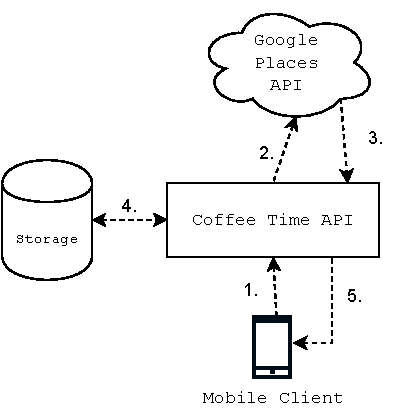
\includegraphics[width=0.5\linewidth]{img/analysis/api-communication-flow.pdf}
    \caption{Client and API communication flow}
    \label{fig:api-communication}
\end{figure}

\begin{enumerate}
    \item HTTP request made by client to Coffee Time API.
    \item The request is processed and redirected to Google Places API.
    \item The response from Google Places API is obtained.
    \item If appropriate the query to storage is issued, and response is enhanced with obtained data.
    \item The final result is returned to the client.
\end{enumerate}
% --- & --- & --- & --- & --- & --- & --- & --- & --- & --- & --- & --- & --- & --- & --- & --- & --- & --- &
\subsubsection{The Cafe Tags}

\begin{figure}[ht]
    \centering
    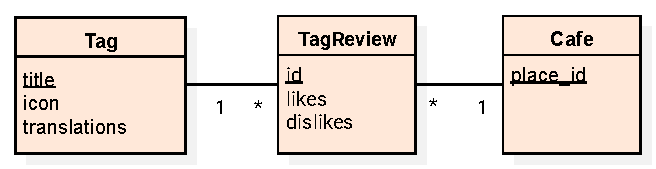
\includegraphics[width=0.8\linewidth]{img/analysis/tag-cafe-relation.pdf}
    \caption{Cafe's tag and Cafe relation}
    \label{fig:tag-cafe-relation}
\end{figure}

The set of available tags is predefined, with the requirement to be able to change it any time without changes within the client or in~the API. Each tag has a~title and icon and can be translated into another language. This definition and requirement for no changes within the client imply that used icon has to be part of tag's definition in the~\gls{cta}. To sum up, each tag is an entity with a unique title, icon and translation. 

As was said earlier in this chapter, each cafe can have assigned tags. Each assigned tag is reviewed by users with the concept of ``likes'' and ``dislikes''.  This requirement implies that for each cafe is needed to be known assigned tags and their reviews. This relation is shown at~\cref{fig:tag-cafe-relation}.
% --- & --- & --- & --- & --- & --- & --- & --- & --- & --- & --- & --- & --- & --- & --- & --- & --- & --- &
\subsubsection{Domain Model}
Within detail screen, additional information is displayed, which can be obtained from the Place Details call. This concludes that the application's cafe domain entity is split into two entities - Cafe and Cafe Detail entities. The~domain entity graph is listed in~\cref{fig:domain} which shows all entities related to~\gls{cta} response.

\begin{figure}[ht]
    \centering
    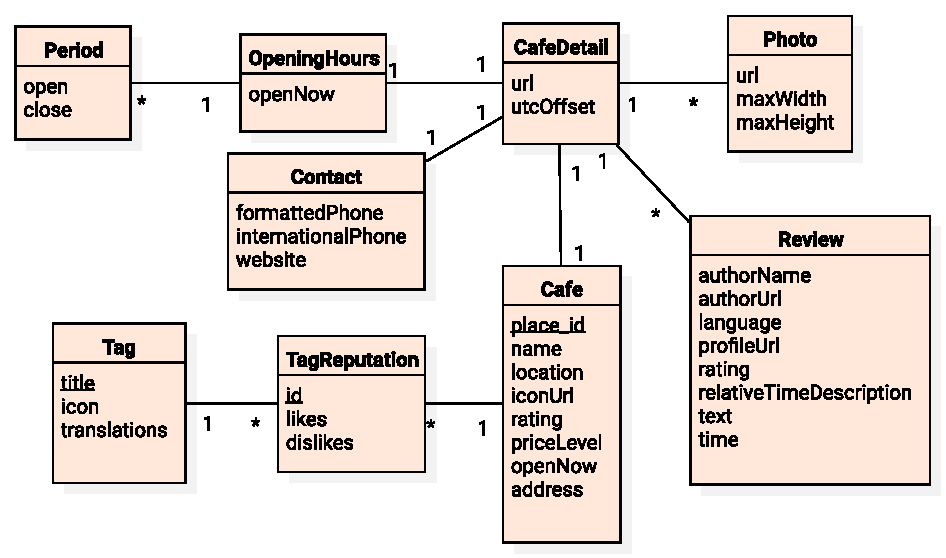
\includegraphics[width=0.9\linewidth]{img/analysis/domain.pdf}
    \caption{Coffee Time domain model}
    \label{fig:domain}
\end{figure}
% --- & --- & --- & --- & --- & --- & --- & --- & --- & --- & --- & --- & --- & --- & --- & --- & --- & --- &
\subsubsection{The API Endpoints}
The~\gls{cta} has endpoints divided into three categories - places, tags and photos. As a client is considered to be multilingual, the API is too. The Places API accepts, as was described earlier, language parameter to specify how the response should be localised. The API is proposed with language parameter in place and required as a mandatory part of the~URI. The tags category offers endpoint for obtaining and manipulating tags. As of last, photo category gives access to downloading the place's photo. Every response coming from \gls{gpa} which returns places are modified such that each ``place'' entry contains additional \verb|tags| field which is an~array of the~\verb|tag| model. 

The~\cref{table:cta-places} describes each API endpoint and its usage. Mandatory parameters within URI are highlighted as \verb|<param>|. Each URI is shown without prefix \verb|http[s]://domain/api| (the hosting url and \verb|/api| suffix).
% -----------------------------
\begin{table}[ht]
\centering
\begin{tabularx}{\textwidth}{|l|l|X|}
\hline
\textbf{URI} & \textbf{HTTP Method} & \textbf{Description} \\ \hline
\verb|<language>/nearby?parameters| & GET & Get nearby cafes \\ \hline
\verb|<language>/find?parameters| & GET & Find cafes within area based on text query \\ \hline
\verb|<language>/detail/<place_id>| & GET & Place's details of given \verb|place_id| \\ \hline
\verb|<language>/basic/<place_id>| & GET & Returns basic place information \\ \hline
\end{tabularx}
\caption{Places endpoints}
\label{table:cta-places}
\end{table}
% -----------------------------
\begin{table}[ht]
\centering
\begin{tabularx}{\textwidth}{|l|l|X|}
\hline
\textbf{Parameter} & \textbf{Required} & \textbf{Description} \\ \hline
\verb|location=lat,lng| & Yes & Location to search, where \verb|lat|=latitude, \verb|lng|=longitude \\ \hline
\verb|radius| & No & If omitted, the results is sorted by \textit{prominence} (see below), otherwise by distance\\ \hline
\verb|opennow| & No & If present returns only opened cafes\\ \hline
\verb|pagetoken| & No & If present, next page returned\\ \hline
\end{tabularx}
\caption{Nearby parameters}
\label{table:cta-nearby-params}
\end{table}

The~\cref{table:cta-nearby-params} describes \textit{nearby} parameter. Note that, if radius is omitted, the results are sorted by Google's ranking -- ``Ranking will favor prominent places within the specified area. Prominence can be affected by a place's ranking in Google's index, global popularity, and other factors''~\cite{google-places-api-nearby-req} otherwise the results are sorted by distance. 
% -----------------------------
\begin{table}[ht]
\centering
\begin{tabularx}{\textwidth}{|l|l|X|}
\hline
\textbf{Parameter} & \textbf{Required} & \textbf{Description} \\ \hline
\verb|input| & Yes & Search query to use \\ \hline
\verb|location=lat,lng| & No & Search within circular area defined by radius \\ \hline
\verb|radius| & No & Circular radius in meters\\ \hline
\end{tabularx}
\caption{Find parameters}
\label{table:cta-find-params}
\end{table}

The~\cref{table:cta-find-params} describes \textit{find} parameters. The \verb|location=lan,lng| and \verb|radius| must be provided both if used. 
% -----------------------------
\begin{table}[ht]
\centering
\begin{tabularx}{\textwidth}{|l|l|X|}
\hline
\textbf{URI} & \textbf{HTTP Method} & \textbf{Description} \\ \hline
\verb|/tags| & GET & Get all defined tags \\ \hline
\verb|/tags/<place_id>| & GET & Get all assigned tags to given \verb|place_id| \\ \hline
\verb|/tags/<place_id>| & POST & Updates tag's review for given \verb|place_id| \\ \hline
\end{tabularx}
\caption{Tags endpoints}
\label{table:cta-tags}
\end{table}

\begin{listing}[ht]
\begin{minted}{json}
[
    {
        "id": "tag",
        "change": "like|dislike"
    }
]
\end{minted}
\caption{Tag update content example}
\label{listing:tag-update-post}
\end{listing}

The~\cref{table:cta-tags} describes all endpoints relative to \textit{tags}. The POST request to \verb|/tags/<place_id>| should have a~body with array of \textit{TagUpdate} model. The example is listed in~\cref{listing:tag-update-post} where \verb|id| contains tag's id and \verb|change| contains value of \verb|like| or \verb|dislike|. More details are described later in~\cref{ch:implementation} about API implementation.

% --- # --- # --- # --- # --- # --- # --- # --- # --- # --- # --- # --- # --- # --- # --- # --- # --- # --- #
\subsection{The Selection of the Right Technology}
The technology which will be used to build the API should fulfil the following requirements

\begin{itemize}
    \item The access to API should be secured
    \item The back-end service should be simply scaled up when needed
    \item The maintenance cost should be kept low
\end{itemize}

There are many technologies which can be used to achieve this requirements. One of the ways is implementing API from the ground with technologies such as \textit{.NET Core} and its \textit{ASP .NET Core API}. Then the~API can be deployed to service hosting providers such as~\textit{Microsoft Azure} or through technologies such as Docker containers and Kubernetes~\cite{kubernetes} as container orchestration. 

Another way is to use serverless services. The serverless is approach where ``the cloud provider is responsible for executing a piece of code by dynamically allocating the resources. And only charging for the amount of resources used to run the code. The code is typically run inside stateless containers that can be triggered by a variety of events including http requests, database events, queuing services, monitoring alerts, file uploads, scheduled events (cron jobs), etc''~\cite{what-is-serverless}. This approach is sometimes called as \textit{Functions as a Service} (FaaS in short). The major providers are \textit{Amazon Web Services} and its \textit{Lambda Functions}, \textit{Microsoft Azure Functions} or \textit{Cloud Functions (Firebase Functions)} by \textit{Google}. 

The~\textit{Firebase} by~\textit{Google} is collection of services which helps to build mobile application faster, improve application quality and grow business. The~\textit{Firebase} offer services as real-time NoSQL database, application usage analytics, A/B user testing, cloud web hosting or Cloud Functions and much more. Within one service, the storage for data, the API as functions and security can be made. 
% --- & --- & --- & --- & --- & --- & --- & --- & --- & --- & --- & --- & --- & --- & --- & --- & --- & --- &
\subsubsection{Cloud Firestore}
\textit{Cloud Firestore} is a flexible, scalable database for mobile, web, and server development. It keeps data in sync across client apps through realtime listeners and offers offline support for mobile and web. The \textit{Cloud Firestore} uses NoSQL data model. The data are stored in documents that contain fields mapping to values. These documents are stored in collections, which are containers for documents that are used to organize data. Documents support many different data types, from simple strings and numbers, to complex, nested objects. Documents can include subcollections and build hierarchical data structures that scale as database grows~\cite{cloud-firestore}.
% --- & --- & --- & --- & --- & --- & --- & --- & --- & --- & --- & --- & --- & --- & --- & --- & --- & --- &
\subsubsection{Cloud Functions}
\textit{Cloud Functions} for \textit{Firebase} is a serverless framework that lets automatically run backend code in response to events triggered by Firebase and HTTPS requests. After function is deployed, Google's servers begin to manage the function immediately. The~function can be used directly with an HTTP request. Each function runs in isolation, in its own environment with its own configuration and are scaled accordingly to usage load~\cite{cloud-functions}. 
% --- & --- & --- & --- & --- & --- & --- & --- & --- & --- & --- & --- & --- & --- & --- & --- & --- & --- &
\subsubsection{Firebase Authentication}
\textit{Firebase Auth} offers service to secure application with \textit{OAuth~2.0} standard~\cite{oauth}. It automatically integrates with identity providers such as \textit{Google}, \textit{Microsoft}, \textit{Facebook} and more. Besides that it offers standard authentication through user's email or phone~\cite{cloud-auth} and anonymous authentication where for each user randomly generated identifier is used. The~service guarantees that for each user, as long they use the same device, the identifier stays the same. 
\\
\\
The~\textit{Cloud Functions} can be used to build Coffee Time API. The~\textit{Cloud Firestore} as a database (storage) and API can be secured through \textit{Firebase Authentication}. On top of that, \textit{Firebase} offers services for analysis, logging and user testing. The~\textit{Firebase} has ``pay as you go'' model and offers a free plan (Spark plan). The Spark plan offers up to 1~GiB data storage, 20~thousands of writes and 50~thousand of document reads per day. The~\textit{Cloud Functions} can be invoked 125~thousand times per month. This pricing perfectly suits the requirements and can be used freely to build Coffee Time application. If the application becomes popular and frequently used, the actual price of \textit{Firebase} services is calculated by current usage and services can be scaled up accordingly. How the \textit{Firebase} services are used in detail is more described in~\cref{ch:implementation}. 

% ----- % ----- % ----- % ----- % ----- % ----- % ----- % ----- % ----- % ----- % ----- % ----- % ----- % ----- %
\section{The Conclusion}
In this chapter, the considered application Coffee Time was introduced. The analysis of existing alternatives was made to obtain inspiration for how each application behaves. The prototype was created to propose user interface and tested it with users. In the end, the analysis of Coffee Time API was made along with analysis of chosen technology to build this API.